\documentclass{mythesis}

\usetikzlibrary{patterns}

% PGFPLOTS STUFF
\usepackage{pgfplots}
\pgfplotsset{compat=1.11}
\usepgfplotslibrary{external}
\tikzexternalize
\pgfplotsset{every axis/.append style={
    no markers
}}
\pgfplotsset{every axis plot/.append style={
    line width=0.6pt
}}
\pgfplotsset{every axis legend/.append style={
    at={(1.02,1)},
    anchor=north west
}}
\definecolor{Set2-8-1}{RGB}{102,194,165}
\definecolor{Set2-8-2}{RGB}{252,141,98}
\definecolor{Set2-8-3}{RGB}{141,160,203}
\definecolor{Set2-8-4}{RGB}{231,138,195}
\definecolor{Set2-8-5}{RGB}{166,216,84}
\definecolor{Set2-8-6}{RGB}{255,217,47}
\definecolor{Set2-8-7}{RGB}{229,196,148}
\definecolor{Set2-8-8}{RGB}{179,179,179}
\pgfplotscreateplotcyclelist{mycolor}{
    {Set2-8-1},
    {Set2-8-2},
    {Set2-8-3},
    {Set2-8-4},
    {Set2-8-5},
    {Set2-8-6},
    {Set2-8-7},
    {Set2-8-8}
}
\pgfplotsset{every axis/.append style={cycle list name=mycolor}}


\DeclareDocumentCommand{\myincludegraphics}{om}{
    \begin{tikzpicture}
	\node[draw=black!30,inner sep=0] {
	    \includegraphics[#1]{#2}
	};
    \end{tikzpicture}
}

\usepackage{titling}

\title{Inpainting mit Eulers Elastica}
\author{Stephan Hilb}


\DeclareDocumentCommand{\P}{}{\mathbb{P}}
\DeclareDocumentCommand{\D}{}{\mathbb{D}}

%\DeclareDocumentCommand{\thesection}{}{\arabic{section}}
%\DeclareDocumentCommand{\thesubsection}{}{\thesection.\arabic{subsection}}

% "such that"
\DeclareDocumentCommand{\st}{}{\mathbin{|}}

\DeclareDocumentCommand{\Edat}{}{E_{\mathrm{dat}}}
\DeclareDocumentCommand{\Eimg}{}{E_{\mathrm{img}}}

\DeclareDocumentCommand{\BV}{}{\mathord{\mathrm{BV}}}

\DeclareDocumentCommand{\Hdiv}{}{H^{\mathrm{div}}}
\DeclareDocumentCommand{\kmax}{}{k_{\mathrm{max}}}

\tikzset{missing/.style={dashed,pattern=checkerboard,pattern color=red!15}}

\colorlet{fg}{black}
\colorlet{bg}{white}


\AtBeginDocument{
    \catcode`_=12
    \begingroup\lccode`~=`_
    \lowercase{\endgroup\let~}\sb
    \mathcode`_="8000
}


\begin{document}

%\usepackage{titling}

\begin{titlepage}
  \begin{center}
    ~\par\vspace{4em}
    {
      \fontsize { 16pt } { 16pt } \selectfont
      Masterarbeit
    }
    \par\vspace{3em}
    {
      \fontsize { 24pt } { 24pt } \selectfont \sffamily \bfseries
      \thetitle
    }
    \par\vspace{3em}
    {
      \fontsize { 16pt } { 16pt } \selectfont \scshape
      \theauthor
    }
    \par\vspace{1.5em}
    {
      \fontsize { 14pt } { 14pt } \selectfont %\scshape
      \today
    }
    \par\vspace{4.5em}
    {
    }
    \par\vspace{8em}
    {
      \fontsize { 14pt } { 14pt } \selectfont \scshape
      Universität Stuttgart
    }
    \par\vspace{1em}
    {
      \fontsize { 14pt } { 14pt } \selectfont %\scshape
      Institut für Angewandte Analysis und Numerische Simulation
    }
    \par\vspace{1em}
    {
      \fontsize { 14pt } { 14pt } \selectfont %\scshape
      Betreuer:
      Dr. Claus J. Heine,
      Dr. Andreas Langer
    }
  \end{center}
\end{titlepage}

\chapter*{Zusammenfassung}

Die Zielsetzung, fehlende Teile eines Bildes zu rekonstruieren – auch „Inpainting“ genannt – lässt sich als Minimierung eines
Funktionals für das Gesamtbild modellieren, bestimmt durch ein Datenmodell, das die Übereinstimmung mit dem ursprünglichen Bild auf dem bekannten Gebiet kontrolliert, und einem Bildmodell, welches maßgebend für die Güte der Rekonstruktion ist.

Das Euler Elastica Bildmodell, welches die Niveaulinien eines Bildes nach dem Vorbild elastischer Stäbe modelliert, bietet ein vielversprechendes Bildmodell und kommt in dieser Arbeit zum Einsatz.
Für die numerische Minimierung wird eine bekannte “alternating direction“ Augmented Lagrange Methode angewandt und die entstehenden Teilprobleme erstmalig im Kontext der Finiten Elemente gelöst.


{
  \let\clearpage\relax
  \tableofcontents
  %\addtocentrydefault{chapter}{}{Inhaltsverzeichnis}
}
%\tableofcontents



\chapter{Einführung} \label{chap:intro}

%
%\begin{itemize}
%    \item
%	Lösungsansätze für das EE inpainting model in der Literatur
%\end{itemize}
%
%Mit Blick auf \ref{fig:setting} führen wir zunächst Begrifflichkeiten ein.


%Die Rekonstruktion fehlender Information ist seit jeher ein verlockendes Forschungsgebiet.
Wir beschäftigen uns in dieser Arbeit mit dem sogenannten „\emph{Inpainting}“, dem Vorgang, verlorengegangene Teile eines Bildes zu rekonstruieren.
Unter Bildern versteht man meistens Fotos und Grafiken, aber auch Skulpturen (als dreidimensionale Bilder) oder Signale (als eindimensionale Bilder).
Mathematisch fassen wir Bilder wie folgt.

\begin{definition} \label{def:image}
    Ein \emphdef{Bild} ist eine Abbildung $u: \Omega \to F$, wobei $\Omega \subset \R^d$
    \emphdef{Trägermenge} genannt wird und $F$ \emphdef{Farbraum}.
    Für einen festen Farbraum $F$ sei $I_\Omega$ die Menge der Bilder mit Trägermenge $\Omega$.
    \begin{note}
	Wir betrachten im weiteren Verlauf Graustufenbilder und setzen daher stets $F := [0,1]$ (mit der
	Interpretation: $0$ entspricht „schwarz“ und $1$ „weiß“).
    \end{note}
\end{definition}

Wann immer man Strukturen oder geometrische Eigenschaften in Bildern untersuchen möchte, ist man dazu geneigt Definition \ref{def:image} einzuschränken indem man z.B. eine Form von Differenzierbarkeit der entsprechenden Abbildungen fordert.
Obwohl dies oft im Widerspruch zu den üblichen Eigenschaften von Bildern steht (z.B. Unstetigkeiten an Kanten und Konturen), werden wir dies später an den entsprechenden Stellen tun.

\begin{figure}[ht]
    \centering
    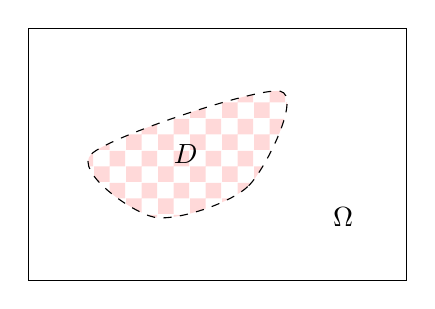
\begin{tikzpicture}[scale=0.8]
	\draw (0,0) rectangle (6,4);
	\draw (5,1) node {$\Omega$};
	\draw[missing] plot[smooth cycle] coordinates {(2,1) (3.5,1.5) (4,3) (1,2)};
	\draw (2.5,2) node {$D$};
    \end{tikzpicture}
    \caption{Typische Inpainting-Situation}
    \label{fig:inpainting_setting}
\end{figure}

Beim Inpainting gehen wir von einem gegebenen Bild $u^0: \Omega \setminus D \to [0,1]$ und einem \emphdef{Inpainting-Bereich}
$D \subset \Omega$ aus (siehe Abbildung \ref{fig:inpainting_setting}). Ziel ist es nun, eine Rekonstruktion $u: \Omega \to [0,1]$ zu finden, die optisch „möglichst gut zu $u^0$ passt“.

Wir werden „möglichst gut“ durch die Minimierung der Summe,
\begin{math}
    \Eimg[u] + \Edat[u]
\end{math}
zweier Funktionale $\Eimg, \Edat: I_\Omega \to \R$ beschreiben.
Die Motivation für dieses Vorgehen und die Interpretation des \emphdef{Bildterms} $\Eimg[u]$ und des \emphdef{Datenterms} $\Edat[u]$ liefert das Bayes'sche Prinzip \cite{chan2005variational,mumford1994bayesian} aus der Wahrscheinlichkeitstheorie.

%bestehend aus zwei Termen: dem 
%beschreiben.
%
%Hierbei sind die Funktionale $\Edat$, $\Eimg$ modelliert durch ein sogenanntes Datenmodell (engl. „data model”) und einem Bildmodell (engl. „image prior model”.
%Der Bayes'sche Ansatz liefert hierfür eine schmackhafte Motivation.
%

\section{Das Bayes'sche Prinzip}

% TODO: fix!!
% TODO: Energiebegriff erklären

Es seien hier $I_\Omega$, $I_{\Omega \setminus D}$ endlich.
Dies ist beispielsweise der Fall, wenn $\Omega \subset \Z^d$ beschränkt und $F$ endlich ist.
Auf praktisch alle digitalen Bilder triftt diese Annahme zu, da in der Regel diese auf einem endlichen Raster $(x_i, y_j)_{i,j=1}^{n,m}$ durch die Angabe von Farbwerten $(u_{i,j})_{i,j=1}^{n,m}$ gegeben sind und der zugehörige Farbraum aus endlich vielen verschiedenen Farbwerten besteht.

\begin{samepage}
Geht man davon aus, dass ein ursprünglich vollständiges Bild $u$ auch tatsächlich existiert, so lässt sich daraus die Entstehung der Beobachtung $u^0$ durch ein zweistufiges Zufallsexperiment modellieren.
\begin{enumerate}
    \item
	Zunächst tritt $u$ als Ereignis eines Zufallsexperiments auf, welches im (diskreten) Wahrscheinlichkeitsraum $(I_\Omega, 2^{I_\Omega}, P_{\mathrm{img}})$ modelliert wird. \nopagebreak
    \item
	Anschließend entsteht von $u$ auf $\Omega \setminus D$ eine Beobachtung $u^0$, welche ebenfalls als Zufallsexperiment modelliert wird,
	hier in $(I_{\Omega \setminus D}, 2^{I_{\Omega \setminus D}}, P_{\mathrm{dat},u})$.
\end{enumerate}
\end{samepage}
Wir betrachten dazu den diskreten Wahrscheinlichkeitsraum $\scr P := (I_\Omega \times I_{\Omega\setminus D}, 2^{I_\Omega \times I_{\Omega\setminus D}}, P)$ mit der sogenannten A-Posteriori-Wahrscheinlichkeitsverteilung
\begin{math}
    P(u, u^0) := P_{\mathrm{img}}(u) \cdot P_{\mathrm{dat},u}(u^0)
\end{math}
In diesem Raum besitzt $P_{\mathrm{dat},u}(u^0)$ die gewünschte Interpretation als bedingte Wahrscheinlichkeit $P(u^0|u)$:
\begin{math}
    P(u) &= P_{\mathrm{img}}(u), \\
    P(u^0|u) &= \frac{P(u^0)}{P(u)} = P_{\mathrm{dat},u}(u^0),
\end{math}
wobei wir $u$ und $u^0$ mit $\Set{u} \times I_{\Omega \setminus D}$, bzw. $I_\Omega \times \Set{u_0}$ identifizieren.
Dieser Raum erlaubt uns die Berechnung der bedingten Wahrscheinlichkeit
\begin{math}
    P(u|u^0) &= \frac{P(u)}{P(u^0)}
    = \frac{P(u^0|u) \cdot P(u)}{P(u^0)}.
\end{math}
Dieser einfache Zusammenhang zwischen den bedingten Wahrscheinlichkeiten ist auch als \emph{Satz von Bayes} bekannt.

Beim Inpainten ist $P(u^0)$ konstant und $P(u|u^0)$ die Wahrscheinlichkeit, dass $u$ die korrekte Rekonstruktion von $u^0$ ist, also \emph{maximieren} wir
\begin{math}
    P(u|u^0) = c \cdot P_{\mathrm{dat},u}(u^0) \cdot P_{\mathrm{img}}(u)
\end{math}
für eine Konstante $c \in \R_{>0}$.
Wir können nun auf beiden Seiten $-\log(\argdot)$ anwenden und äquivalent den folgenden Ausdruck \emph{minimieren}:
\begin{math}
    -\log(P(u|u^0)) = \underbrace{-\log(P_{\mathrm{dat},u}(u^0))}_{=:E_{\mathrm{img}}[u]} \underbrace{-\log(P_{\mathrm{img}}(u))}_{=:E_{\mathrm{dat}}[u]} - \log(c).
\end{math}
Für gegebenes $u^0$ und $D$ minimieren wir also (bis auf additive Konstanten) die Summe $\Eimg[u] + \Edat[u]$

Die Wahl von Bildterm $\Eimg[u]$ und Datenterm $\Edat[u]$ entsprechen also der Modellierung der obigen Zufallsexperimente:
das \emphdef{Bildmodell} beschreibt die Entstehung von $u$, während das \emphdef{Datenmodell} die Beobachtung $u^0$ aus $u$ beschreibt.
Beide Modelle zusammen bilden das \emphdef{Inpainting-Modell}.
Im Folgenden legen wir das Bild- und das Datenmodell für unsere Zwecke fest.


%Die Wahl der Wahrscheinlichkeitsverteilungen $P_{\mathrm{img}}$, $P_{\mathrm{dat},u}$, bzw. die Wahl von Bild- und Datenterm $\Eimg[u]$, $\Edat[u]$ 

%ein äquivalentes, aber durchaus handlicheres Problem in Energie-Form betrachten.
%
%Für gegebenes $u^0$, $D$ minimieren wir also die Summe aus Datenterm und Bildterm (die additive Konstante ist für das Minimieren irrelevant)
%\begin{math}
%    E[u] = \Edat[u] + \Eimg[u].
%\end{math}
%
%Die Wahlen von $\Edat[u]$ und $\Eimg[u]$, welche den Wahrscheinlichkeitsverteilungen in unserem zweistufigen Zufallsmodell entsprechen, sind durch das Datenmodell, bzw. das Bildmodell festgelegt.
%

\section{Das Datenmodell}

Das Datenmodell legt fest, wie $u^0$ als Beobachtung der ursprünglichen Bildes $u$ auf $\Omega \setminus D$ hervorgegangen ist.
Naheliegend ist der Gedanke, als Datenmodell lediglich $u^0|_{\Omega \setminus D} = u|_{\Omega \setminus D}$ zu fordern, d.h. die Beobachtung $u^0$ von $u$ ist genau $u$ eingeschränkt auf $\Omega \setminus D$.
%Damit würden feste Randbedingungen für das Minimieren auf $D$ vorgegeben werden.
In der Praxis sind Bilder jedoch meist mit Rauschen, Unschärfe oder anderen Artefakten versehen.
Dies kann z.B. durch technische Aufnahmebedingungen, natürlichen Zerfall oder durch digitale Kompression verursacht worden sein.
Das Datenmodell erlaubt es zu definieren, auf welche Weise $u|_{\Omega \setminus D}$ beim Inpainten an das vorliegende Bild $u^0$ angepasst werden soll und ermöglicht es solche Verunreinigungen auszugleichen.

Für $D = \emptyset$ reduziert sich das Inpaintingproblem auf das reine Ausgleichen dieser Verunreinigungen.
Somit kann z.B. das Entrauschen von Bildern (auch „Denoising“ genannt) als Spezialfall angesehen werden.

Wir modellieren für unser Datenmodell $u^0|_{\Omega \setminus D} = u|_{\Omega \setminus D} + \epsilon$ für additives Gauß'sches Rauschen $\epsilon$, d.h. in jedem Punkt $x \in \Omega\setminus D$ ist die Wahrscheinlichkeit für ein Rauschen $\epsilon(x) = \epsilon_x \in \R$ durch die Gauß-Verteilung
\begin{math}[numbered] \label{eq:gnoise}
    p(\epsilon_x) = \frac{1}{\sigma \sqrt{2\pi}} e^{-\frac{\epsilon_x^2}{2\sigma^2}}
\end{math}
mit Varianz $\sigma^2$ gegeben.
Wir maximieren also
\begin{math}
    P_{\mathrm{dat},u}(u^0) = \frac{1}{|\Omega\setminus D|}\int_{\Omega\setminus D} p(\epsilon_x) \di[x],
\end{math}
wobei $\epsilon_x := u^0(x) - u(x)$ das aktuelle Rauschen an der Stelle $x$ angibt.
Äquivalent minimieren wir also
\begin{math}[numbered] \label{eq:edat}
    \Edat[u] &:= - \log \Big(\frac{1}{|\Omega\setminus D|}\int_{\Omega\setminus D} \frac{1}{\sigma \sqrt{2\pi}} e^{-\frac{(u^0(x) - u(x))^2}{2\sigma^2}} \di[x] \Big) \\
    &= -\log \big(\sigma \sqrt{2\pi}|\Omega\setminus D|\big) + \frac{1}{2\sigma^2} \underbrace{\int_{\Omega\setminus D} |u(x) - u^0(x)|^2 \di[x]}_{=\|u^0 - u\|_{L^2(\Omega\setminus D)}}.
\end{math}
Bis auf Gewichtung und additive Konstanten handelt es sich also um die quadrierte $L^2$-Norm von $u - u^0$ auf $\Omega \setminus D$, welche auch in \cite{rudin1992nonlinear} genutzt wird.


%Für unser Datenmodell nutzen wir das bekannte Funktional aus \cite{rudin1992nonlinear}, welcher die quadrierte $L^2$-Norm verwendet:
%\begin{math}
%    \Edat[u] = \frac{\eta}{2} \int_{\Omega \setminus D} |u - u^0|^2,
%\end{math}
%wobei $\eta \in \R_{> 0}$ die spätere Gewichtung dieses Datenterms zum Bildterm kontrolliert.
%
%Es ist bekannt \cite[§4.5]{chan2005image}, dass dieser Datenterm gut geeignet ist, wenn das Orginalbild mit weißem Gauß'schem Rauschen versetzt ist, modelliert als $u^0 = u|_{\Omega \setminus D} + \epsilon$.
%Man kann dies folgendermaßen motivieren.
%
%Für additives weißes Gauß'sches Rauschen gibt die Gauß-Verteilung
%\begin{math}[numbered] \label{eq:gnoise}
%    p(\epsilon_x) = \frac{1}{\sigma \sqrt{2\pi}} e^{-\frac{\epsilon_x^2}{2\sigma^2}}
%\end{math}
%an jeder Stelle $x \in \Omega$ des Bildes die Wahrscheinlichkeit dafür, dass das Rauschen $\epsilon_x$ beträgt.

Für Schwarz/Weiß Rauschen (auch „salt-and-pepper noise” gennant) ist die Wahl einer $L^1$-Norm zu bevorzugen, wie in \cite{nikolova2004variational} gezeigt.

Denkbar wären auch Datenmodelle wie $u^0|_{\Omega\setminus D} = K[u|_{\Omega\setminus D}] + \epsilon$ für einen Glättungsoperator $K$ und additives Rauschen $\epsilon$.
Solche Modelle würden es z.B. erlauben, Unschärfe zu reduzieren, siehe z.B. \cite{rudin1994total}.


\section{Das Bildmodell}

Das Bildmodell beschreibt die Enstehung des ursprünglichen Bildes $u$.
Es ist bestimmt durch die Klasse von Bildern, von denen man erwartet, dass sie als ursprüngliche Bilder beim Inpainting auftreten.

Da der Datenterm sich auf $\Omega \setminus D$ beschränkt hat, trägt das Bildmodell die Hauptrolle bei der eigentlichen Bildrekonstruktion innerhalb von $D$.
Man beachte, dass das Bildmodell unabhängig von $D$ ist (mit Blick auf das Bayes-Prinzip) und auch für den Fall $D = \emptyset$ (z.B. Denoising) die Rekonstruktion des ursprünglichen Bildes verbessern kann.
In der Literatur zum Denoising wird $\Eimg[u]$ manchmal auch als \emph{Regularisierungsterm} bezeichnet.

\begin{figure}[ht]
    \begin{subfigure}[b]{0.33\textwidth}
	\centering
        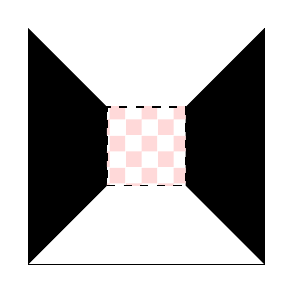
\begin{tikzpicture}
	    \draw[clip] (0,0) rectangle (3,3);
	    \fill[bg] (0,0) rectangle (3,3);
	    \fill[fg] (0,0) -- (1,1) -- (1,2) -- (0,3) -- cycle;
	    \fill[fg] (3,0) -- (3,3) -- (2,2) -- (2,1) -- cycle;
	    \draw[missing] (1,1) -- (2,1) -- (2,2) -- (1,2) -- cycle;
        \end{tikzpicture}
    \end{subfigure}%
    \begin{subfigure}[b]{0.33\textwidth}
	\centering
        
\begin{tikzpicture}
	    \draw[clip] (0,0) rectangle (3,3);
	    \fill[fg] (0,0) rectangle (3,3);
	    \fill[bg] (0,0) -- (3,0) -- (2,1) -- (1,1) -- cycle;
	    \fill[bg] (0,3) -- (1,2) -- (2,2) -- (3,3) -- cycle;
        \end{tikzpicture}
    \end{subfigure}%
    \begin{subfigure}[b]{0.33\textwidth}
	\centering
        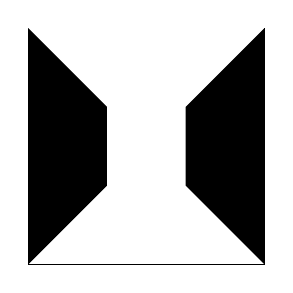
\begin{tikzpicture}
	    \draw[clip] (0,0) rectangle (3,3);
	    \fill[bg] (0,0) rectangle (3,3);
	    \fill[fg] (0,0) -- (1,1) -- (1,2) -- (0,3) -- cycle;
	    \fill[fg] (3,0) -- (3,3) -- (2,2) -- (2,1) -- cycle;
        \end{tikzpicture}
    \end{subfigure}
    \caption{Bewertungsschwierigkeiten: welches der beiden vollständigen Bildern ist wahrscheinlicher?}
    \label{fig:inpainting_non_unique}
\end{figure}

Zunächst macht man sich schnell anhand von einfachen Beispielen klar, dass die Wahl eines guten Bildmodells keineswegs einfach oder eindeutig ist, da die Bildbewertung oft von der menschlichen Interpretation abhängt.
Welche der beiden vollständigen Bilder aus Abbildung \ref{fig:inpainting_non_unique} ein Betrachter eher für richtig hält, hängt davon ab, ob er Hell oder Dunkel für vordergründiger hält.

\begin{figure}[ht]
    \begin{subfigure}[b]{0.33\textwidth}
	\centering
        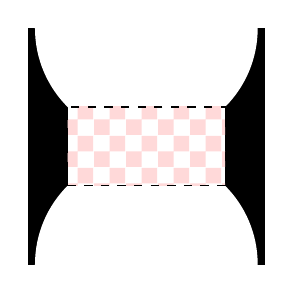
\begin{tikzpicture}
	    \draw[clip] (0,0) rectangle (3,3);
	    \fill[fg] (0,0) rectangle (3,3);
	    \fill[bg] (1.5,3) circle[radius=1.41421];
	    \fill[bg] (1.5,0) circle[radius=1.41421];
	    \fill[bg] (0.5,1) -- (2.5,1) -- (2.5,2) -- (0.5,2) -- cycle;
	    \draw[missing] (0.5,1) -- (2.5,1) -- (2.5,2) -- (0.5,2) -- cycle;
        \end{tikzpicture}
    \end{subfigure}%
    \begin{subfigure}[b]{0.33\textwidth}
	\centering
        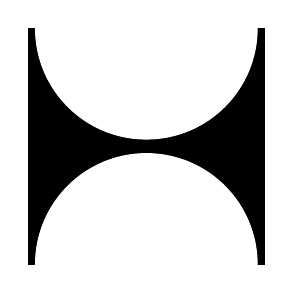
\begin{tikzpicture}
	    \draw[clip] (0,0) rectangle (3,3);
	    \fill[fg] (0,0) rectangle (3,3);
	    \fill[bg] (1.5,3) circle[radius=1.41421];
	    \fill[bg] (1.5,0) circle[radius=1.41421];
        \end{tikzpicture}
    \end{subfigure}%
    \begin{subfigure}[b]{0.33\textwidth}
	\centering
        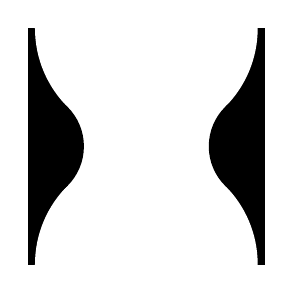
\begin{tikzpicture}
	    \draw[clip] (0,0) rectangle (3,3);
	    \fill[fg] (0,0) rectangle (3,3);
	    \fill[bg] (1.5,3) circle[radius=1.41421];
	    \fill[bg] (1.5,0) circle[radius=1.41421];
	    \fill[bg] (0.5,1) -- (2.5,1) -- (2.5,2) -- (0.5,2) -- cycle;
	    \fill[fg] (0,1.5) circle[radius=0.70710];
	    \fill[fg] (3,1.5) circle[radius=0.70710];
        \end{tikzpicture}
    \end{subfigure}
    \caption{Lösungen eines Inpaintingproblems (links) mit langen (mitte) und kurzen (rechts) Niveaulinien}
    \label{fig:inpainting_prefer_short}
\end{figure}

%\begin{figure}[ht]
%    \begin{subfigure}[b]{0.33\textwidth}
%	\centering
%        \begin{tikzpicture}
%	    \draw[clip] (0,0) rectangle (3,3);
%	    \fill[fg] (0,0) rectangle (3,3);
%	    \fill[bg] (1.5,3) circle[radius=1.11803];
%	    \fill[bg] (1.5,0) circle[radius=1.11803];
%	    \fill[bg] (1,1) -- (2,1) -- (2,2) -- (1,2) -- cycle;
%	    \draw[missing] (1,1) -- (2,1) -- (2,2) -- (1,2) -- cycle;
%        \end{tikzpicture}
%    \end{subfigure}%
%    \begin{subfigure}[b]{0.33\textwidth}
%	\centering
%        \begin{tikzpicture}
%	    \draw[clip] (0,0) rectangle (3,3);
%	    \fill[fg] (0,0) rectangle (3,3);
%	    \fill[bg] (1.5,3) circle[radius=1.11803];
%	    \fill[bg] (1.5,0) circle[radius=1.11803];
%        \end{tikzpicture}
%    \end{subfigure}%
%    \begin{subfigure}[b]{0.33\textwidth}
%	\centering
%        \begin{tikzpicture}
%	    \draw[clip] (0,0) rectangle (3,3);
%	    \fill[fg] (0,0) rectangle (3,3);
%	    \fill[bg] (1.5,3) circle[radius=1.11803];
%	    \fill[bg] (1.5,0) circle[radius=1.11803];
%	    \fill[bg] (1,1) -- (2,1) -- (2,2) -- (1,2) -- cycle;
%	    \fill[fg] (0.75,1.5) circle[radius=0.55902];
%	    \fill[fg] (2.25,1.5) circle[radius=0.55902];
%        \end{tikzpicture}
%    \end{subfigure}
%    \caption{Krümmungsarme Niveaulinien (mitte) werden bevorzugt}
%    \label{fig:inpainting_prefer_non_curved}
%\end{figure}

\begin{figure}[ht]
    \begin{subfigure}[b]{0.33\textwidth}
	\centering
        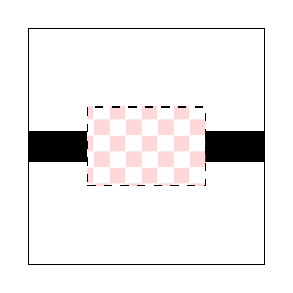
\begin{tikzpicture}
	    \draw[clip] (0,0) rectangle (3,3);
	    \fill[fg] (0,1.3) rectangle (3,1.7);
	    \fill[bg] (0.75,1) -- (2.25,1) -- (2.25,2) -- (0.75,2) -- cycle;
	    \draw[missing] (0.75,1) -- (2.25,1) -- (2.25,2) -- (0.75,2) -- cycle;
        \end{tikzpicture}
    \end{subfigure}%
    \begin{subfigure}[b]{0.33\textwidth}
	\centering
        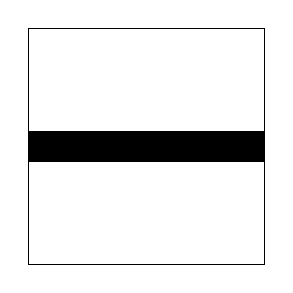
\begin{tikzpicture}
	    \draw[clip] (0,0) rectangle (3,3);
	    \fill[fg] (0,1.3) rectangle (3,1.7);
        \end{tikzpicture}
    \end{subfigure}%
    \begin{subfigure}[b]{0.33\textwidth}
	\centering
        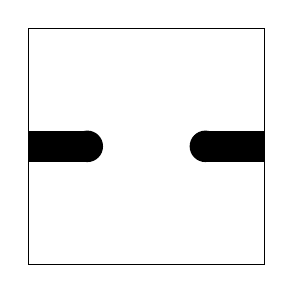
\begin{tikzpicture}
	    \draw[clip] (0,0) rectangle (3,3);
	    \fill[fg] (0,1.3) rectangle (3,1.7);
	    \fill[bg] (0.75,1) -- (2.25,1) -- (2.25,2) -- (0.75,2) -- cycle;
	    \fill[fg] (0.75,1.5) circle[radius=0.2];
	    \fill[fg] (2.25,1.5) circle[radius=0.2];
        \end{tikzpicture}
    \end{subfigure}
    \caption{Lösungen eines Inpaintingproblems (links) mit Nivaulinien ohne Krümmung (mitte) und Niveaulinien höherer Krümmung (rechts)}
    \label{fig:inpainting_prefer_non_curved}
\end{figure}

Ein allgemeines Bildmodell kann (ohne sich der Stochastik zu bedienen) empirisch durch ästhetische Ansprüche an das Inpainting-Resultat gewonnen werden.
Ohne entsprechende Studien durchgeführt zu haben, kann man anhand von Abbildungen \ref{fig:inpainting_prefer_short} und \ref{fig:inpainting_prefer_non_curved} erahnen, dass Bilder, bei denen die Kanten (oder Niveaulinien) des Bildes möglichst kurz und gering gekrümmt sind, als Inpainting-Resultate zu bevorzugen sind.

Die Niveaulinien stellen auf diese Weise eine brauchbare Bewertungsgrundlage eines Bildes dar.
Legt man nun eine geeignete Bewertung für die Niveaulinien eines Bildes (im Sinne eines Energiefunktionals) fest, so liefert die Summation über alle Höhenlinien eine Bewertung des Gesamtbildes.

Das Bildmodell in dieser Arbeit nutzt diese sogenannte \emphdef{Levelset-Methode} (siehe Kapitel \ref{chap:image_model}) und wählt als Bewertung für jede Niveaulinie $\gamma:[0,1] \to \Omega$ die \emphdef{Elastica Energie}
\begin{math}
    \int_{\gamma} \alpha + \beta \kappa^2 \di[s]
\end{math}
als Kurvenintegral über $\gamma$ mit festen Parametern $\alpha \in \R_{>0}$, $\beta \in \R_{\ge 0}$, wobei $\kappa: [0,1] \to \R$ die parametrisierte Krümmung von $\gamma$ darstellt.

Eine Kurve, die diese Energie (unter geeigneten Randbedingungen) minimiert, wird \emphdef{Elastica} genannt.
In der Physik hat sie die Interpretation der Biegeenergie eines elastischen Stabes.
Umfangreiche Herleitungen finden sich in \cite{antman2005problems,love1920treatise}, während obige Form der Elastica Energie aus \cite{birkhoff1965nonlinear} stammt.

Die Levelset-Methode liefert uns schließlich für unser Bildmodell (näheres in Kapitel \ref{chap:image_model})
\begin{math}
    \Eimg[u] = \int_{\Omega} \Big(\alpha + \beta (\nabla \cdot \frac{\nabla u(x)}{\nabla u(x)})^2\Big)|\nabla u(x)| \di[x],
\end{math}
wobei der Term $\nabla \cdot \frac{\nabla u}{|\nabla u|}$ die Krümmung der Niveaulinie im entsprechenden Punkt darstellt.
Der Bildterm $\Eimg[u]$ entstammt bei dieser Wahl nicht einer entsprechenden Wahrscheinlichkeitsverteilung $\P_{\mathrm{img}}[u]$.

Mit Blick auf Abbildung \ref{fig:inpainting_texture} sei bemerkt, dass dieses geometrische Inpaintingmodell nicht darauf ausgelegt ist, wiederkehrende Strukturen zu reproduzieren, die deutlich kleiner als der Inpaintingbereich $D$ sind.
Die Minimierung einer Energie basierend auf Niveaulinien und der Levelset-Methode ist in diesem Fall nicht zielführend, da sie eine zu lokale Methode darstellt.
Um solche Strukturen oder Texturen zu rekonstruieren, müssen größere Teile des Bildes in Betracht gezogen werden.
Hierfür gibt es das sogenannte „texture based inpainting” mit zahlreichen stochastischen Methoden (siehe z.B. \cite{criminisi2004region}).

\begin{figure}[ht]
    \begin{subfigure}[b]{0.33\textwidth}
	\centering
        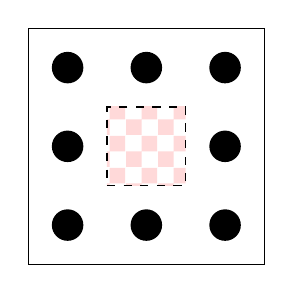
\begin{tikzpicture}
	    \draw[clip] (0,0) rectangle (3,3);
	    \foreach \x in {0.5, 1.5, 2.5}
		\foreach \y in {0.5, 1.5, 2.5}
		    \fill (\x,\y) circle[radius=0.2];
	    \fill[bg] (1,1) -- (2,1) -- (2,2) -- (1,2) -- cycle;
	    \draw[missing] (1,1) -- (2,1) -- (2,2) -- (1,2) -- cycle;
        \end{tikzpicture}
    \end{subfigure}%
    \begin{subfigure}[b]{0.33\textwidth}
	\centering
        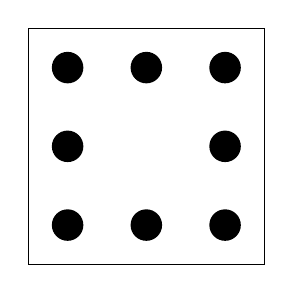
\begin{tikzpicture}
	    \draw[clip] (0,0) rectangle (3,3);
	    \foreach \x in {0.5, 1.5, 2.5}
		\foreach \y in {0.5, 1.5, 2.5}
		    \fill (\x,\y) circle[radius=0.2];
	    \fill[bg] (1,1) -- (2,1) -- (2,2) -- (1,2) -- cycle;
        \end{tikzpicture}
    \end{subfigure}%
    \begin{subfigure}[b]{0.33\textwidth}
	\centering
        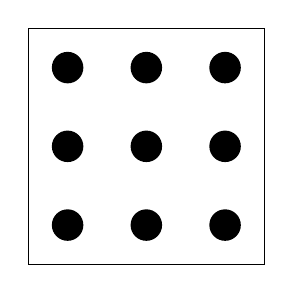
\begin{tikzpicture}
	    \draw[clip] (0,0) rectangle (3,3);
	    \foreach \x in {0.5, 1.5, 2.5}
		\foreach \y in {0.5, 1.5, 2.5}
		    \fill (\x,\y) circle[radius=0.2];
        \end{tikzpicture}
    \end{subfigure}
    \caption{Unser Bildmodell würde das mittlere Bild dem rechten vorziehen}
    \label{fig:inpainting_texture}
\end{figure}

\section{Ausblick}

Unser Inpainting-Modell besteht also aus der Minimierung der Summe des $L^2$-Datenterms $\Edat[u]$ und dem Elastica Bildterm $\Eimg[u]$.
Bis auf additive Konstanten minimieren wir daher
\begin{math}
    E[u] := \int_\Omega \Big(\alpha + \beta ( \nabla \cdot \frac{\nabla u(x)}{|\nabla u(x)|})^2 \Big) |\nabla u(x)| \di[x]
    + \frac{\eta}{2} \int_{\Omega\setminus D} |u(x) - u^0(x)|^2 \di[x].
\end{math}
Hierbei gewichtet $\eta \in \R_{>0}$ den Datenterm im Verhältnis zum Bildterm.
Einen Zusammenhang von $\eta$ mit $\frac{1}{2\sigma^2}$ aus \eqref{eq:edat} ist nicht direkt gegeben, da der Bildterm $\Eimg[u]$ nicht unbedingt zu einem Wahrscheinlichkeitsmaß $P_{\mathrm{img}}(u)$ gehört: die Parameter $\alpha$ und $\beta$ können die Gewichtung des Bild- und des Datenterms ebenfalls beeinflussen.

Ziel dieser Arbeit war die Implementierung einer sogenannten „alternating direction“ Augmented Lagrange Methode aus \cite{tai2011fast} für Elastica Inpainting, d.h. zur Minimierung von $E[u]$.
Dabei sollten statt der Finiten Differenzen Diskretisierung in \cite{tai2011fast} eine Diskretisierung mit Finiten Elementen erfolgen und im C++ Framework Dune \cite{dune-web-page,blatt2016distributed} implementiert werden.

In Kapitel \ref{chap:technical} werden wir einige technischen Hilfsmittel vorstellen, sowie Konventionen festlegen, die im Laufe der Arbeit genutzt werden.
Die Herleitung des Bildterms $\Eimg[u]$ aus dem Elastica Kurvenmodell erfolgt in Kapitel \ref{chap:image_model}.
In Kapitel \ref{chap:adm} wird der „alternating direction“ Augmented Lagrange Algorithmus motiviert und vorgestellt, während in Kapitel \ref{chap:numerics} die numerische Implementierung und die erhaltenen Resultate präsentiert werden.


\chapter{Technische Hilfsmittel und Konventionen} \label{chap:technical}


\section*{Konventionen}

Um die Notation zu erleichtern, werden wir eine Reihe von Konventionen befolgen, die im Folgenden festgehalten werden sollen.

\begin{itemize}
    \item
	Bei Integralen einer Funktion $f: X \to Y$ über Teilmengen des Definitionsbereiches von $f$ wird das Funktionsargument ausgespart, z.B. $\int_X f \dx$.
    \item
	Bei Integralen über Teilmengen des $\R^d$ wird das Integrationsmaß ausgespart, falls es sich um das übliche Lebesgue-Maß handelt.
    \item
	Für Vektorfelder $v, w: X \to \R^d$ (oder Vektoren) bezeichnen wir mit $v \cdot w$ das (punktweise) euklidische Skalarprodukt von $v$ und $w$ und mit $|v|$ die (punktweise) euklidische Norm von $v$.
    \item
	Für Funktionen $f, g \in H$ eines Hilbertraums $H$ bezeichen wir mit $\<f, g\>_H$ das zugehörige Skalarprodukt von $f$ und $g$ und mit $\|f\|_H$ die entsprechende Norm von $f$.
    \item
	Für einen Funktionenraum $H$ bezeichnen wir Funktionen $I: H \to \R$ als \emphdef{Funktionale} und schreiben ihr Argument stets in eckigen Klammern: $I[f] \in \R$ für $f \in H$.
    \item
	Für Kurven $\gamma: [0,1] \to \R^d$ notieren wir die Ableitung nach der Parametrisierungsvariable mit einem Punkt: $\dot \gamma(t) = \ddx[t] \gamma(t)$.
    \item
	Für ein Minimierungsproblem der Form „Minimiere $f(x)$ für $x \in X$ unter der Nebenbedingung $e(x) = 0$“ schreiben wir kurz
	\begin{math}
	    \min_{x\in X} f(x) \quad \mathrm{u.d.N.} \quad e(x) = 0.
	\end{math}
\end{itemize}


\section*{Differentialgeometrie}

Sei $\gamma \in C^2([0,L], \R^2)$ eine nach Bogenlänge parametrisierte Kurve.
Außerdem sei $\gamma$ \emphdef{regulär}, d.h. $|\dot\gamma| > 0$ auf $[0,L]$.

Die Tangente $e_1 \in C^1([0,L], \R^2)$ und Normale $e_2 \in C^1([0,L], \R^2)$ von $\gamma$ sind gegeben durch
\begin{math}
    e_1(t) := \dot\gamma(t), \qquad
    e_2(t) := e_1^{\orth}(t) = \Matrix{0 & -1 \\ 1 & 0} e_1(t).
\end{math}
Wegen $|e_1|^2 = 1$, ergibt sich durch Ableiten
\begin{math}
    0 = \ddx[t] e_1(t) \cdot e_1(t)
    = 2 \dot e_1(t) \cdot e_1(t),
\end{math}
also haben wir punktweise eine lineare Abhängigkeit $\dot e_1 = \kappa e_2$ für eine skalare Funktion $\kappa: [0,L] \to \R$, genannt \emphdef{Krümmung} von $\gamma$.
Wegen $0 = \ddx[t] e_1(t) \cdot e_2(t) = \dot e_1(t) \cdot e_2(t) + \dot e_2(t) \cdot e_1(t)$ folgern wir also
\begin{math}
    \Vector*{\dot e_1 & \dot e_2}
    = \Matrix*{0 & \kappa \\ -\kappa & 0} \Vector*{e_1 & e_2},
\end{math}
die sogenannten \emphdef{Frenet-Gleichungen} in $\R^2$, welche wir in Kapitel \ref{chap:image_model} nutzen werden.
Die Frenet-Gleichungen existieren auch für Raumkurven in höheren Dimensionen, siehe \cite{kuhnel2013differentialgeometrie}.

Wir haben folgende wohlbekannte parametrisierungsunabhängige Darstellung für die Krümmung einer regulären Kurve.
\begin{lemma}
    Sei $\gamma \in C^2([0,1], \R^2)$ eine reguläre Kurve.
    Dann ist ihre Krümmung $\kappa: [0,1] \to \R$ gegeben durch
    \begin{math}
	\kappa = \dfrac{\det(\dot\gamma, \ddot\gamma)}{|\dot\gamma|^3}.
    \end{math}
    \begin{proof}
	Sei $\gamma = c \circ \phi$ mit einer nach Bogenlänge parametrisierten Kurve $c:[0,L] \to \R^2$ und einer Parametertransformation $\phi: \R \to \R$.
	Mit $e_1$ und $e_2$ bezeichnen wir Tangente und Normale von $c$.
	Wir berechnen die Krümmung $\kappa = \kappa_c \circ \phi$ von $\gamma$, wobei $\kappa_c$ die Krümmung von $c$ ist.
        Es gilt zunächst
	\begin{math}
	    \dot \gamma &= (\dot c \circ \phi)\dot\phi, \qquad
	    \ddot \gamma = (\ddot c \circ \phi) \dot\phi^2 + (\dot c \circ \phi) \ddot\phi, \\
	    |\dot\gamma| &= \dot \phi.
	\end{math}
	Also
	\begin{math}
	    \det(\dot\gamma, \ddot\gamma)
	    &= \dot\phi^3 \det( \dot c \circ \phi, \ddot c \circ \phi) \\
	    &= |\dot\gamma|^3 \det(e_1 \circ \phi, \dot e_1 \circ \phi)
	    = |\dot\gamma|^3 (\kappa_c \circ \phi),
	\end{math}
	wie behauptet.
    \end{proof}
\end{lemma}


\section*{Optimierung}

Wir nutzen in Kapitel \ref{chap:image_model} und \ref{chap:adm} Variationsrechnung im Zusammenhang mit Optimierung und führen dazu kurz die nötigen Werkzeuge ein.
Im Folgenden sei $H$ stets ein Hilbertraum.

\begin{definition} \label{definition:min_stuff}
    Wir nennen $I: H \to \R$
    \begin{itemize}
	\item
	    \emphdef{Gâteaux-differenzierbar} in $u \in H$,
            falls für alle $\phi \in H$ das \emphdef{Gâteaux-Differential $I': H \times H \to \R$ von $I$ an der Stelle $u$ in Richtung $\phi$}
	    \begin{math}
		I'[u, \phi]
		:= \ddx[\epsilon]|_{\epsilon = 0} I[u + \epsilon \phi]
		= \lim_{\delta \to 0} \dfrac{I[u + \delta \phi] - I[u]}{\delta}
	    \end{math}
	    existiert und $I'[u, \argdot]: H \to \R$ ein linearer und beschränkter Operator ist,
	\item
	    \emphdef{Fréchet-differenzierbar} in $u \in H$,
	    falls für alle $\phi \in H$ ein Operator $I': H \times H \to \R$ existiert – genannt \emphdef{Fréchet-Differential} – sodass
	    \begin{math}
		\lim_{\|\phi\| \to 0} \dfrac{\|I[u+\phi] - I[u] - I'[u,\phi]\|}{\|\phi\|} = 0
	    \end{math}
	    und $I'[u,\argdot]: H \to \R$ ein linearer und beschränkter Operator ist.
        \item
	    \emphdef{konvex},
	    falls für alle $u_1, u_2 \in H$, $t \in [0,1]$ gilt
	    \begin{math}
		I[t u_1 + (1-t) u_2]
		\le tI[u_1] + (1-t)I[u_2],
	    \end{math}
	\item
	    \emphdef{koerziv},
	    falls für jede Folge $(u_k)_{k\in\N}$ gilt
	    \begin{math}
		\|u_k\| \to \infty \implies I(u_k) \to \infty.
	    \end{math}
    \end{itemize}
\end{definition}

Der folgende aus der Optimierung bekannte Satz rechtfertigt das Ermitteln von kritischen Punkten eines Funktionals, um sein Minimum zu bestimmen.

\begin{proposition} \label{prop:mincrit}
    Sei $\hat u \in H$ und $I: H \to \R$ Gâteaux-differenzierbar und konvex.
    Dann gilt
    \begin{math}
        I[\hat u] = \inf_{u \in H} I[u]
	\iff
	\forall \phi \in H : I'[\hat u, \phi] = 0.
    \end{math}
    \begin{note}
	Über die Lösbarkeit von $I'[u, \phi] = 0$ für alle $\phi$, bzw. die Existenz des Minimums $\hat u$ wird hier keine Aussage getroffen, siehe dazu Theorem \ref{thm:minexist}.
    \end{note}
    \begin{proof}
	„$\implies$”: Sei $I[\hat u] \le I[u]$ für alle $u \in H$.
	Dann gilt für alle $\phi \in H$
	\begin{math}
	    I'[\hat u, \phi] = \lim_{\epsilon \to 0} \frac{I[\hat u + \epsilon \phi] - I[\hat u]}{\epsilon}
	    \ge 0,
	\end{math}
	also auch $-I'[\hat u, \phi] = I'[\hat u, -\phi] \ge 0$ und somit $I'[\hat u, \phi] = 0$.

	„$\impliedby$”: Sei $I'[\hat u, \phi] = 0$ für alle $\phi \in H$.
	Wegen Konvexität haben wir
	\begin{math}
	    0 = I'[\hat u, u - \hat u]
	    &= \lim_{\epsilon \to 0} \frac{1}{\epsilon} \big( I[\epsilon u + (1-\epsilon) \hat u] - I[\hat u] \big) \\
	    &\le \lim_{\epsilon \to 0} \frac{1}{\epsilon} \big( \epsilon I[u] + (1- \epsilon) I[\hat u] - I[\hat u] \big) \\
	    &= I[u] - I[\hat u],
	\end{math}
	also $I[\hat u] \le I[u]$ für alle $u \in H$.
    \end{proof}
\end{proposition}

\begin{theorem} \label{thm:minexist}
    Sei $I: H \to \R$ Gâteaux-differenzierbar, konvex und koerziv.
    Dann existiert ein Minimum $\hat u \in H$, d.h.
    \begin{math}
        I[\hat u] = \inf_{u \in H} I[u].
    \end{math}
    \begin{proof}
        Ein Beweis für eine etwas allgemeinere Version findet sich in \cite[Theorem 7.3.8]{kurdila2006convex}.
    \end{proof}
\end{theorem}

Die obigen beiden Aussagen sind für die Minimierung von konvexen Funktionalen von wesentlicher Bedeutung.

Die sogenannte \emphdef{Euler-Lagrange-Gleichung} macht die Suche nach einem kritischen Punkt eines Funktionals der Form
\begin{math}
    I[u] := \int_\Omega f(x,u(x),\nabla u(x)) \di[x]
\end{math}
etwas leichter.
Hierbei sei $\Omega \subset \R^d$ ein $C^1$-berandetes Gebiet, $f \in C^2(\Omega, \R, \R^d)$ und $u \in C^1(\Omega)$ mit natürlicher Randbedingung $\partial_\nu u|_{\Boundary \Omega} = 0$.

Durch den Ansatz $0 = \ddx[\epsilon]|_{\epsilon=0} I[u + \epsilon\phi]$ erhält man nach geeigneter Variationsrechnung die Bedingung
\begin{math}
    \nabla_x \cdot (\nabla_3 f(x, u, \nabla u)) = \partial_2 f(x,u,\nabla u),
\end{math}
wobei $\partial_2 f$, $\nabla_3 f$ die Ableitungen bezüglich der zweiten und dritten Komponente von $f$ darstellen und $\nabla_x \cdot (\dotsc)$ die Divergenz nach $x \in \Omega$.
Für nähere Ausführungen sei auf \cite[§8.1]{evans2010partial} verwiesen.
Wir werden in dieser Arbeit den variationellen Ansatz stets explizit führen und benötigen die Euler"=Lagrange"=Gleichung daher nicht.

Zur Untersuchung der nötigen Voraussetzungen für Satz \ref{prop:mincrit} und Theorem \ref{thm:minexist} für spätere Zwecke folgen zwei einfache, konkretere Lemmata.

\begin{lemma} \label{lem:convexity}
    Für Funktionale $I: H \to \R$ gelten folgende Aussagen über ihre Konvexität.
    \begin{enumerate}[i)]
	\item
	    Konstante Funktionale sind konvex.
	\item
	    Lineare Funktionale sind konvex.
        \item
	    Die Summe zweier konvexer Funktionale ist konvex.
	\item
	    Seien $\Omega \subset \R^d$ und $H := L^2(\Omega)^d$.
	    Seien $A: H \to H$ ein linearer Operator, $v \in H$ und $w \in L^1(\Omega)$ sodass $w|Au + v|^2 \in L^1(\Omega)$.
	    Dann ist das Funktional
	    \begin{math}
	        I: u \mapsto \int_\Omega w|Au + v|^2
	    \end{math}
	    konvex.
    \end{enumerate}
    \begin{proof}
	Die Aussagen i), ii) und iii) sind mit Blick auf Definition \ref{definition:min_stuff} sofort ersichtlich, wir zeigen nur iv).

	Sei $I: u \mapsto \int_\Omega w|Au + v|^2$ für einen linearen Operator $A$.
	Wegen
	\begin{math}
	    |Au - v|^2
	    = |Au|^2 - 2Au \cdot v + |v|^2
	\end{math}
	genügt es mit Blick auf i), ii) und iii) den Fall $v = 0$ zu betrachten.
	Es folgt mit $t^2 = t - t(1-t)$ punktweise fast überall
	\begin{math}
	    |A(tu_1 + (1-t)u_2)|^2
	    &= t^2 |Au_1|^2 - 2 t(1-t) Au_1\cdot Au_2 + (1-t^2)|Au_2|^2 \\
	    &= t|Au_1|^2 - t(1-t)\underbrace{\big(|Au_1|^2 - 2Au_1 \cdot Au_2 + |Au_2|^2\big)}_{=|A(u_1 - u_2)|^2 \ge 0} + (1-t)|Au_2|^2 \\
	    &\le t|Au_1|^2 + (1-t)|Au_2|^2,
	\end{math}
	also wegen Distributivität der Multiplikation und Linearität des Integrals auch $I[tu_1 + (1-t)u_2] \le tI[u_1] + (1-t)I[u_2]$.
    \end{proof}
\end{lemma}

\begin{lemma} \label{lem:coercivity}
    Für Funktionale $I: H \to \R$ gelten folgende Aussagen über ihre Koerzivität:
    \begin{enumerate}[i)]
        \item
	   Die Summe zweier koerziver Funktionale ist koerziv.
       \item
	   Sei $I: H \to \R$ koerziv und $J: H \to \R$ nach unten beschränkt.
	   Dann ist $I + J$ koerziv.
       \item
	   Seien $\Omega \subset \R^d$, $H := L^2(\Omega)^d$, $v, w \in H$.
	   Dann ist das Funktional
	   \begin{math}
	       I: u \mapsto \int_\Omega |u - v|^2 + \int_\Omega u \cdot w
	   \end{math}
	   koerziv.
    \end{enumerate}
    \begin{proof}
	Die Aussagen i) und ii) sind mit Blick auf Definition \ref{definition:min_stuff} leicht ersichtlich und wir zeigen nur iii).
	Durch quadratische Ergänzung und mit Hilfe von ii) genügt es den Fall $w = 0$ zu betrachten.
	Hierfür ist
	\begin{math}
	    I[u] = \int_\Omega |u - v|^2 = \|u - v\|^2 \ge (\|u\| - \|v\|)^2,
	\end{math}
	also für eine Folge $\|u_k\| \to \infty$ auch $I[u_k] \to \infty$.
    \end{proof}
\end{lemma}

\section*{Sobolev-Räume}

Zur Analyse der Koerzivität in Kapitel \ref{chap:adm} benötigen wir folgende Form der wohlbekannten Poincaré Ungleichung.

\begin{theorem}[Poincaré-Wirtinger] \label{thm:poincare-wirtinger}
    Sei $\Omega \subset \R^d$ offen, zusammenhängend und beschränkt mit $C^1$-Rand $\Boundary \Omega$.
    Dann gilt für alle $u \in H^1(\Omega)$
    \begin{math}
	\|u - t\|_{L^2(\Omega)} \le c \cdot \|\nabla u\|_{L^2(\Omega)},
    \end{math}
    wobei $t := \frac{1}{|\Omega|} \int_\Omega u$ der Mittelwert von $u$ auf $\Omega$ ist und die Konstante $c \in \R_{\ge 0}$ nur von $\Omega$ abhängt.
    \begin{proof}
        Für einen Beweis sei auf \cite[§5.8.1]{evans2010partial} verwiesen.
    \end{proof}
\end{theorem}

Für Funktionale der Form $\int_\Omega (\nabla \cdot n)^2 + \int_\Omega |n|^2$ setzen wir den Raum $\Hdiv(\Omega)^d$ der Funktionen an, deren schwache Divergenz quadratintegrierbar ist.

\begin{definition}[{\normalfont\scshape\cite[Definition 3.5]{kurula2012duality}}] \label{def:hdiv}
    Sei $\Omega \subset \R^d$ offen.
    Wir definieren den Funktionenraum
    \begin{math}
	\Hdiv(\Omega) := \Set{u \in L^2(\Omega, \R^d) & \nabla \cdot u \in L^2(\Omega)},
    \end{math}
    wobei $\nabla \cdot u = \sum_{i=0}^d \partial_i u$ mit schwachen partiellen Ableitungen $\partial_i u$.
\end{definition}

\begin{proposition}[{\normalfont\scshape\cite[Lemma 3.6]{kurula2012duality}}] \label{lem:hdivhilbert}
    Der Raum $\Hdiv(\Omega)$ bildet zusammen mit dem Skalarprodukt
    \begin{math}
	\<u, v\>_{\Hdiv(\Omega)} := \<u, v\>_{L^2(\Omega)^d} + \<\nabla \cdot u, \nabla \cdot v\>_{L^2(\Omega)}
    \end{math}
    einen Hilbertraum.
\end{proposition}


\section*{Finite Elemente}

Für die Diskretisierung in Kapitel \ref{chap:numerics} werden wir an dieser Stelle die entsprechenden diskreten Funktionenräume kurz festhalten.
Die folgenden Definitionen entstammen weitestgehend \cite{haasdonk2014enumpde,heine2016fem}.

\begin{definition}
    Ein \emphdef{Dreieck} $T$ sei die konvexe Hülle dreier affin linearer Punkte in $\R^2$.
    Für ein Dreieck $T$ sei
    \begin{math}
	\P_k(T) := \Big\{p: T \to \R \;\Big|\; p(x) = \sum_{s \in \N_0^2, |s| \le k} a_s x^s, a_s \in \R \Big\}
    \end{math}
    der Raum der polynomiellen Funktionen auf $T$.

    Eine Menge $\scr T := \Set{T_i}_{i=1}^n$ von Dreiecken nennen wir \emphdef{Triangulierung} einer offenen Menge $\Omega \subset \R^2$, falls
    \begin{itemize}
        \item
	    $\bigcup_{i=1}^n T_i = \_\Omega$ und
	\item
	    $\mathring T_i \cap \mathring T_j = \emptyset$ für alle $i \neq j$.
    \end{itemize}
    Wir nennen $\scr T$ \emphdef{konform}, falls alle Dreiecke in $\scr T$ paarweise disjunkt sind, oder sich in genau einer gemeinsamen Seite schneiden.
    Weiter sei $\scr T$ \emphdef{uniform}, falls alle Dreiecke in $\scr T$ paarweise kongruent sind.

\end{definition}

\begin{definition}
    Für eine Triangulierung $\scr T$ von $\Omega \subset \R^2$ definieren wir den Raum der global stetigen, stückweise polynomiellen Funktionen
    \begin{math}
	\P_k(\scr T) := \Set{p \in C^0(\_\Omega) & \forall T \in \scr T : p|_{T} \in \P_k(T)},
    \end{math}
    wobei $\P_k(T)$ den Raum der polynomiellen Funktionen von Grad $k$ auf $T$ bezeichnet.
\end{definition}

\begin{definition}
    Für eine Triangulierung $\scr T$ von $\Omega \subset \R^2$ definieren wir den Raum der diskontinuierlichen, stückweise polynomiellen Funktionen
    \begin{math}
	\D_k(\scr T) := \Set{p \in L^1(\Omega) & \forall T \in \scr T : p|_T \in \P_k(T) \text{ fast überall}}.
    \end{math}
\end{definition}











\chapter{Das Euler Elastica Bildmodell} \label{chap:image_model}


Wie bereits in der Einführung angesprochen, wollen wir in diesem Kapitel die Elastica Kurve als Kurvenmodell für die Niveaulinien eines Bildes ansetzen, um daraus anschließend ein Bildmodell zu gewinnen.
Obwohl das hieraus gewonnene Bildmodell später auch für $d > 2$ interpretiert werden kann (siehe Definition \ref{def:eemodel}), werden wir uns für die Herleitung auf die Dimension $d = 2$ festlegen.

\section{Die Euler Elastica}

In der Physik bezeichnet man einen festen Gegenstand in der Regel als elastisch, wenn er sich unter äußerer Krafteinwirkung deformiert und nach dem Entfernen dieser Kraft wieder in seine Ausgangsform zurückkehrt.
Die Frage, wie genau sich ein elastischer Gegenstand unter äußerer Krafteinwirkung verformt, ist im Allgemeinen stark materialabhängig und schwierig zu beantworten.

Die Wissenschaft hat mit der Zeit mathematische Modelle entwickelt, um das Verhalten elastischer Gegenstände zu beschreiben.
Man erinnere sich beispielsweise an das Hookesche Gesetz aus der Schulphysik, welches zwischen Elongation eines Objektes (z.B. eine Spannfeder) in eine Richtung und der darauf einwirkenden Kraft einen linearen Zusammenhang herstellt.
Dieses Modell war jedoch eindimensional und reichte auch nicht aus, um größere Verformungen zu beschreiben, die sich nicht dem linearen Gesetz unterwerfen.

Euler hat (nach Vorarbeit von Bernoulli und anderen, siehe \cite{levien2008elastica}) 1744 in seinem Buch über variationelle Methoden \cite{euler1774methodus} ein Modell für planare elastische Stäbe fester Länge präsentiert.
Eine Elastica war demnach (in aktueller Notation) eine zweifach stetig differenzierbare, reguläre Kurve $\gamma: [0,1] \to \R^2$ fester Länge $L > 0$, festen Endpunkten $\gamma(0), \gamma(1)$ und festen Tangentenrichtungen $\dot \gamma(0), \dot \gamma(1)$, welche die totale quadrierte Krümmung
\begin{math}
    \int_\gamma \kappa^2 \di[s]
\end{math}
minimiert.
In seinem Werk löst Euler dieses Variationsproblem indem er alle zugehörigen kritischen Punkte (Kurven) klassifiziert und weist darauf hin, dass das Modell bekannte Eigenschaften elastischer Stäbe reproduziert.

Durch ihre Formulierung erbt die Elastica auch viele geometrische Eigenschaften der Krümmung, wie z.B. Invarianz unter euklidischen Transformationen.
In neuerer Zeit wurde die Elastica deshalb in der Numerik z.B. als Vorbild für Spline-Interpolationen oder – wie in dieser Arbeit – als Kurvenmodell für Levelsetmethoden in Betracht gezogen.
Man möchte dabei in der Regel die Länge der Kurve variabel halten und wählt folgende Definition.

\begin{definition}[Euler Elastica] \label{definition:elastica}
    Seien $\alpha \in \R_{>0}, \beta \in \R_{\ge 0}$.
    Eine reguläre Kurve $\gamma \in C^2([0,1], \R^2)$ mit festen Endpunkten $\gamma(0) = p_0$, $\gamma(1) = p_1$ und Tangentenrichtungen $\dot\gamma(0) = t_0$, $\dot\gamma(1) = t_1$ heißt \emphdef{Elastica}, falls sie unter eben solchen zulässigen Kurven ein kritischer Punkt des Funktionals
    \begin{math}
	\int_\gamma \alpha + \beta \kappa^2 \di[s]
    \end{math}
    ist.
    Diese Energie nennen wir auch \emphdef{Elastica Energie der Kurve $\gamma$}.
    \begin{note}
	Es gilt
	\begin{math}
	    \int_\gamma \alpha + \beta \kappa^2 \di[s] = \alpha L + \beta \int_\gamma \kappa^2 \di[s]
	\end{math}
	für die Länge $L$ von $\gamma$.
	Daher sind die Minimierer der Elastica Energie anschaulich bestimmt durch das Verhältnis $\frac{\beta}{\alpha}$.
       	Kleines $\frac{\beta}{\alpha}$ gewichtet die Länge der Kurve stärker und es werden kürzere Verbindungsstrecken bevorzugt, während größeres $\frac{\beta}{\alpha}$ die totale quadrierte Krümmung stärker gewichtet ein glatteres Gesamtbild der Kurve erzeugt.
	In Kapitel \ref{chap:numerics} wird diese Eigenschaft am zugehörigen Inpaintingresultat sichtbar.
    \end{note}
\end{definition}

Eine interessante Charakterisierung der Elastica liefert der folgende Satz.

\begin{proposition} \label{proposition:elastica_el}
    Eine Kurve $\gamma \in C^4([0,1], \R^2)$ mit Randbedingungen wie in Definition \ref{definition:elastica} ist eine Elastica genau dann, wenn die zugehörige Euler-Lagrange-Gleichung für die Krümmung
    \begin{math}
	\beta\big(2\ddot\kappa + \kappa^3\big) = \alpha\kappa
    \end{math}
    erfüllt ist.
    \begin{proof}
	Sei $\gamma:[0,L] \to \R^2$ in Bogenlänge parametrisiert und ebenso ihre Tangente $e_1$, Normale $e_2$ und Krümmung $\kappa$.
        Das Elastica Energiefunktional sei gegeben durch $I[\gamma] := \int_\gamma \alpha + \beta \kappa^2 \di[s]$.
	Wir bedienen uns der Variationsrechnung und lösen
	\begin{math}
	    \ddx[\epsilon]|_{\epsilon=0} I[\gamma + \epsilon \phi e_2] = 0,
	\end{math}
	für alle Variationen $\phi \in C^2([0,L], \R)$ mit entsprechenden Randbedingungen $\phi(0), \phi(L) = 0$, $\dot\phi(0), \dot\phi(L) = 0$.
       	Hier ist also $\phi e_2$ eine Variation in Normalenrichtung $e_2$ von $\gamma$.

	Sei $\gamma_\epsilon = \gamma + \epsilon \phi e_2$.
	Die Krümmung $\kappa_\epsilon$ von $\gamma_\epsilon$ lässt sich parametrisierungsunabhängig durch $\kappa_\epsilon = \frac{\det(\dot\gamma_\epsilon, \ddot\gamma_\epsilon)}{|\dot\gamma_\epsilon|^3}$ darstellen.
	Wir berechnen nun
	\begin{math}
	    \dot \gamma_\epsilon &= e_1 + \epsilon \dot \phi e_2 - \epsilon \phi \kappa e_1 \\
	    &= (1-\epsilon \phi \kappa)e_1 + \epsilon \dot \phi e_2, \\
	    \ddot \gamma_\epsilon &= (-\epsilon \dot \phi \kappa - \epsilon \phi \dot \kappa) e_1 + (1-\epsilon \phi \kappa) \kappa e_2 + \epsilon \ddot \phi e_2 - \epsilon \dot \phi \kappa e_1 \\
	    &= (-2\epsilon \dot\phi \kappa - \epsilon \phi \dot \kappa) e_1 + (\epsilon \ddot \phi - \epsilon \phi \kappa^2 + \kappa) e_2, \\
	    \det(\dot\gamma_\epsilon, \ddot \gamma_\epsilon)
	    &=(1-\epsilon\phi\kappa)(\epsilon\ddot\phi - \epsilon\phi\kappa^2 + \kappa) + \epsilon \dot\phi(2 \epsilon \dot\phi \kappa - \epsilon\phi\dot\kappa),
	\end{math}
	und somit
	\begin{math}
	    \ddx[\epsilon]|_{\epsilon=0} |\dot\gamma_\epsilon|
	    &= \frac{1}{|\dot\gamma_0|} (\dot\gamma_0 \cdot \ddx[\epsilon] \dot\gamma_\epsilon) \\
	    &= e_1 \cdot (-\phi \kappa e_1 + \dot \phi e_2) \\
	    &= - \phi \kappa, \\
	    \ddx[\epsilon]|_{\epsilon=0} \det(\dot\gamma_\epsilon, \ddot\gamma_\epsilon)
	    &= -\phi \kappa^2 + (\ddot \phi - \phi\kappa^2) + \dot\phi \cdot 0 + 0 \cdot (2\dot\phi\kappa + \phi \dot\kappa) \\
	    &= \ddot\phi + 2\phi\kappa^2.
	\end{math}
	Zusammen ergibt sich
	\begin{math}
	    0 &= \ddx[\epsilon]|_{\epsilon = 0} I[\gamma_\epsilon] \\
	    &= \ddx[\epsilon]|_{\epsilon=0} \int_0^L (\alpha + \beta \kappa_\epsilon^2)|\dot\gamma_\epsilon|  \\
	    &= \int_0^L \alpha \ddx[\epsilon]|_{\epsilon = 0}|\dot\gamma_\epsilon| + \beta \ddx[\epsilon]|_{\epsilon = 0} \dfrac{\det(\dot\gamma_\epsilon, \ddot\gamma_\epsilon)^2}{|\dot\gamma_\epsilon|^5}  \\
	    &= \int_0^L -\alpha \kappa \phi + \beta \Big(2\kappa \ddx[\epsilon]|_{\epsilon=0} \det(\dot\gamma_\epsilon, \ddot\gamma_\epsilon) + 5\kappa^3 \phi \Big) \\
	    &= \int_0^L 2\beta\kappa \ddot\phi + \beta \kappa^3 \phi - \alpha\kappa\phi.
	\end{math}
	Zweimalige partielle Integration unter Beachtung der Randbedingungen $\phi(0), \phi(1), \dot\phi(0), \dot\phi(L) = 0$ liefert
	\begin{math}
	    0 &= \int_0^L \Big(2\ddot\kappa + \beta \kappa^3 - \alpha\kappa \Big) \phi
	\end{math}
	und mit dem Hauptsatz der Variationsrechnung also
	\begin{math}
	    \beta(2\ddot\kappa + \kappa^3) - \alpha \kappa = 0.
	\end{math}
    \end{proof}
\end{proposition}

%TODO: kinetische Betrachtung


\section{Die Levelset-Methode}

Die Idee der Levelset-Methode in der Numerik ist es, Berechnungen auf Kurven (oder Flächen) mit Hilfe einer sogenannten Levelset-Funktion in kartesischen Koordinaten durchführen zu können, ohne jeweils eine konkrete Parametrisierung der Kurven zu benötigen.
Die Levelset-Funktion enthält dabei die zu betrachtenden Kurven als Niveaulinien.

\begin{definition}
    Sei $\Omega \subset \R^2$ offen, $\gamma \in C^1([0,1], \Omega)$ eine reguläre Kurve und $\lambda \in \R$.
    Eine stetig differenzierbare Abbildung $u: \Omega \to \R^2$ heißt \emphdef{$\lambda$-Levelset-Funktion} für $\gamma$, falls für alle $t \in [0,1]$ gilt
    \begin{enumerate}[i)]
        \item
	    $(u \circ \gamma)(t) = \lambda$ und
	\item
	    $\det(\dot \gamma(t), \nabla u(\gamma(t))) > 0$.
    \end{enumerate}
    Wir nennen $\gamma$ auch \emphdef{$\lambda$-Levelset-Kurve} zu $u$.
    \begin{note}
        Die zweite Bedingung $\det(\dot \gamma, \nabla u) > 0$ sichert uns eine einheitliche Orienterung der Kurve.
    \end{note}
\end{definition}

Viele von $\gamma$ abhängige Größen können nun auch durch $u$ dargestellt werden, wie z.B. die Einheitsnormale $e_2$ von $\gamma$ an einem Punkt $x = \gamma(t)$.
Einmaliges Ableiten von $(u \circ \gamma)(t) = \lambda$ nach $t$ liefert nämlich
\begin{math}
    0 = \nabla u(\gamma(t)) \cdot \dot \gamma(t).
\end{math}
Falls $\nabla u(x) \neq 0$, so muss also $\frac{\nabla u(x)}{|\nabla u(x)|} = e_2(t)$, wobei das Vorzeichen durch $\det(\dot\gamma, \nabla u) > 0$ sichergestellt ist.
Dies motiviert folgende Definition.

\begin{definition}
    Für eine Abbildung $u \in C^1(\Omega, [0,1])$ mit $\nabla u(x) \neq 0$ für alle $x \in \Omega$ sei
    \begin{math}
        n: \Omega &\to \R^2 \\
	x &\mapsto \frac{\nabla u(x)}{|\nabla u(x)|}
    \end{math}
    das \emphdef{Normalenfeld} von $u$.
\end{definition}

Die Elastica Energie $\int_\gamma \alpha + \beta \kappa^2 \di[s]$ im Hinterkopf, wollen wir nun die Krümmung $\kappa$ der Niveaulinie eines Bildes durch $u$ darstellen.

\begin{lemma}
    Sei $\Omega \subset \R^2$, $\gamma \in C^2([0,1], \Omega)$ regulär und $u \in C^2(\Omega, [0,1])$ eine zugehörige Levelset-Funktion mit Normalenfeld $n: \Omega \to \R^2$ und $\nabla u \neq 0$ auf $\Omega$.
    Dann gilt für alle $t \in [0,1]$, $x := \gamma(t)$
    \begin{math}
	\kappa(t) = - \nabla \cdot n(x) = - \nabla \cdot \frac{\nabla u(x)}{|\nabla u(x)|}.
    \end{math}
    \begin{note}
	Allgemeiner beschreibt $\nabla \cdot n$ in beliebiger Dimension die mittlere Krümmung einer Hyperfläche mit Normale $n$, siehe \cite[§1]{giga2002surface}.
    \end{note}
    \begin{proof}
        Seien $e_1, e_2$ die Einheitstangente und Einheitsnormale von $\gamma$,
       	dann gilt für die Krümmung $\kappa$ nach den Frenet-Gleichungen
	\begin{math}
	    \Vector*{\dot e_1 & \dot e_2} = \Matrix*{0 & \kappa \\ -\kappa & 0} \Vector*{e_1 & e_2}.
	\end{math}
	Wegen $e_2 = n \circ \gamma$ erhalten wir gemäß Kettenregel
	\begin{math}
	    \kappa = - \dot e_2 \cdot e_1 = -n' e_1 \cdot e_1.
	\end{math}
	Außerdem zeigt sich durch Differenzieren von $|n|^2 = n_1^2 + n_2^2 = 1$
	\begin{math}
	    n_1 \partial_1 n_1 + n_2 \partial_1 n_2 &= 0, \\
	    n_1 \partial_2 n_1 + n_2 \partial_2 n_2 &= 0.
	\end{math}
	Zusammen ergibt sich
	\begin{math}
	    -\kappa &= n' e_1 \cdot e_1 \\
	    &= \Matrix*{\partial_1 n_1 & \partial_2 n_1 \\ \partial_1 n_2 & \partial_2 n_2}
	       \Vector*{n_2 & -n_1} \cdot \Vector*{n_2 & -n_1} \\
	    &= n_2 (n_2 \partial_1 n_1 - n_1 \partial_2 n_1) - n_1 (n_2 \partial_1 n_2 - n_1 \partial_2 n_2) \\
	    &= n_2 (n_2 \partial_1 n_1 + n_2 \partial_2 n_2) + n_1 (n_1 \partial_1 n_1 + n_1 \partial_2 n_2) \\
	    &= (n_1^2 + n_2^2) (\partial_1 n_1 + \partial_2 n_2) \\
	    &= \nabla \cdot n,
	\end{math}
	also $\kappa = - \nabla \cdot n$.
    \end{proof}
\end{lemma}

Wir haben damit folgende Darstellung für die Elastica Energie einer Kurve $\gamma$ mit Levelset-Funktion $u$ für den Fall $\nabla u \neq 0$ fast überall:
\begin{math}
    \int_\gamma \alpha + \beta (\nabla \cdot \frac{\nabla u}{|\nabla u|})^2 \di[s].
\end{math}
Um nun ein Funktional für das Gesamtbild zu erhalten, werden wir über alle Levelset-Kurven summieren.
Das Werkzeug dafür ist die sogenannte Coarea-Formel \cite[§3.4]{evans2015measure}, welche wir hier für Levelset-Kurven formulieren.

\begin{proposition}[Coarea-Formel für glatte Bilder] \label{satz:coarea}
    Sei $f \in L^1(\Omega, \R)$ und seien $\gamma_\lambda \in C^1([0,1], \Omega)$ $\lambda$-Levelset-Kurven zu einem Bild $u \in C^1(\Omega, [0,1])$, sodass $\im \gamma_\lambda = \Set{x & u(x) = \lambda}$.
    Dann gilt
    \begin{math}
	\int_0^1 \int_{\gamma_\lambda} f \circ \gamma_\lambda \di[s] \di[\lambda]
	= \int_\Omega f |\nabla u| \di[x].
    \end{math}
    \begin{note}
        Durch entsprechende Zerlegung des Gebiets und wegen der Additivität der Integrale können wir hiermit auch Fälle abdecken, bei denen die Levelsets aus mehreren (fast überall) disjunkten Kurven bestehen.
    \end{note}
    \begin{proof}
        Für eine wesentlich allgemeinere Formulierung mit Beweis, siehe \cite[§3.4]{evans2015measure}.
    \end{proof}
\end{proposition}


\section{Das Euler Elastica Inpaintingmodell}


Die Coarea-Formel motiviert nun die folgende Definition der Euler Elastica Bildenergie.

\begin{definition} \label{def:eemodel}
    Für $u \in C^2(\Omega, [0,1])$ mit $\nabla u \neq 0$ auf $\Omega$ ist das \emphdef{Euler Elastica Bildmodell} festgelegt durch die Minimierung der \emphdef{Elastica Bildenergie}
    \begin{math}
	\int_\Omega \Big(\alpha + \beta (\nabla \cdot \frac{\nabla u}{|\nabla u|})^2\Big)|\nabla u| \di[x].
    \end{math}
    \begin{note}
	\begin{itemize}
	    \item
		In der Regel ignoriert man die Forderung nach $\nabla u \neq 0$ und nutzt die Konvention, dass in diesem Fall der Integrand gleich null ist.
	    \item
		Obige Formulierung ließe sich prinzipiell auch für $\Omega \subset \R^d$ mit $d > 2$ lesen.
		Anmerkungen dazu finden sich in \cite{ambrosio2003direct}.
	    \item
		Man kann diese Energie durch geeignete Methoden auch auf $L^1(\Omega, [0,1])$ erweitern, wie in \cite{ambrosio2003direct}:
		\begin{math}
		    \_E[u] := \inf \Set{ \liminf_{C^2 \ni u_h \to u} E[u_h] }.
		\end{math}
	\end{itemize}
    \end{note}
\end{definition}

\begin{remark}[TV-Bildmodell]
    Aus dem Elastica Bildmodell erhält man für $\alpha = 1, \beta = 0$ das bekannte TV-Bildmodell, welches für ein Bild $u \in C^1(\Omega, [0,1])$ die \emphdef{totale Variation}
    \begin{math}
	V_\Omega[u] := \int_\Omega |\nabla u| \di[x]
    \end{math}
    minimiert.
    Mit Blick auf die Coarea-Formel entsteht dieses Bildmodell aus einem Kurvenmodel, welches die Energie $\int_\gamma \di[s] = L(\gamma)$, d.h. die Länge der entsprechenden Kurven minimiert.
    Einen Vergleich zwischen TV- und Elastica-Inpainting werden wir in Kapitel \ref{chap:numerics} sehen können.

    Das TV-Modell wird unter anderem zum Entrauschen von Bildern verwendet, da es – anders als z.B. Glättungsmethoden – die Kanten eines Bildes gut erhält, wie in \cite{rudin1992nonlinear} beschrieben.
    In der Regel wird die Energie im allgemeineren Raum der Funktionen mit beschränkter totaler Variation
    \begin{math}
	\BV(\Omega) := \Set{u \in L^1(\Omega, [0,1]) & V_\Omega[u] < \infty}.
    \end{math}
    minimiert, wobei die totale Variation $V_\Omega(u)$ hier folgende Form hat (siehe \cite[§2.2]{chan2005image}):
    \begin{math}
	V_\Omega[u] := \sup\Set{ \int_\Omega u \nabla \cdot \phi & \phi \in C_0^1(\Omega,\R^d), \|\phi\|_{L^\infty(\Omega)} \le 1}.
    \end{math}
    Der Raum $\BV$ wird in Bildverarbeitung verwendet, da er im Gegensatz zu $C^1$ oder $H^1$ auch Unstetigkeiten (motiviert durch Kanten in Bildern) zulässt, siehe \cite[§2.2]{chan2005image}.
    %allgemein genug ist, um fast alle konventionellen Bilder zu beschreiben und gleichzeitig hinreichend viel geometrische Struktur bietet, um sinnvolle Bildmodelle zu definieren, näheres in \cite[§2.2]{chan2005image}.
\end{remark}

Erinnert man sich an das Bayes-Prinzip, so steht nun unser Inpaintingmodell fest.

\begin{definition} \label{def:ee_inpainting}
    Für gegebenes $u^0 \in L^2(\Omega, [0,1])$ und Inpaintingbereich $D \subset \Omega$ mit $|\Omega \setminus D| > 0$ ist das \emphdef{Euler Elastica Inpaintingmodell} festgelegt durch die Minimierung der \emphdef{Elastica Inpaintingenergie}
    \begin{math}[numbered] \label{eq:energy_ee}
        E[u] &= \int_\Omega \Big(\alpha + \beta (\nabla \cdot \frac{\nabla u}{|\nabla u|})^2\Big)|\nabla u| \di[x]
	  + \frac{\eta}{2} \int_{\Omega\setminus D} |u - u^0|^2 \di[x]
    \end{math}
    über $u \in C^2(\Omega, [0,1])$ für Konstanten $\beta \in \R_{\ge 0}$, $\alpha,\eta \in \R_{>0}$.
    Der erste Integrand sei dabei Null, falls $\nabla u(x) = 0$.
\end{definition}


\chapter{Die „alternating direction” Methode} \label{chap:adm}


\section{Motivation} % komplexität von euler-lagrange und numerische probl.


Für die numerische Implementierung des Elastica Inpaintingmodells aus Definition \ref{def:ee_inpainting} gibt es verschiedene Ansätze (siehe z.B. \cite{ballester2001filling,brito2010fast,shen2002euler,duan2013fast,hahn2011fast,tai2011fast,yashtini2015alternating}), darunter eine Zeitschrittmethode aus \cite{shen2002euler}, die wir im Folgenden kurz vorstellen und eine „alternating direction“ Augmented Lagrange Methode aus \cite{tai2011fast}, mit der wir uns im Anschluss näher auseinandersetzen werden.

Die Methode aus \cite{shen2002euler} besteht darin, direkt die zugehörige Euler-Lagrange-Gleichung zu ermitteln (meist mit geeigneter Regularisierung, z.B. $\frac{\nabla u}{|\nabla u|} \leadsto \frac{\nabla u}{\sqrt{|\nabla u|^2 + \epsilon^2}}$) und hieraus ein zeitabhängiges Problem zu kreieren.
Sei dazu $\Phi(u) = 0$ die Euler-Lagrange-Gleichung für einen geeigneten Operator $\Phi$.
Dann lautet das zeitabhängige Problem
\begin{math}
    \pddx[t] u = \Phi(u).
\end{math}
Es ist klar, dass eine stationäre (d.h. zeitunabhängige) Lösung dieses Problems auch eine Lösung von $\Phi(u) = 0$ ist.
Durch geeignete Diskretisierung erhält man auf diese Weise ein iteratives Verfahren zur Lösung des Elastica Inpaintingmodells.
In \cite{shen2002euler} werden für diese Diskretisierung finite Differenzen vierter Ordnung benötigt, was das Verfahren rechentechnisch aufwändig macht.

In \cite{tai2011fast} wird ein anderer Algorithmus vorgestellt und dessen Konvergenz numerisch untersucht.
Dabei wird das unrestringierte Minimierungsproblem aus Definition \ref{def:ee_inpainting} durch geeignetes Einführen zusätzlicher Variablen und Nebenbedingungen in ein restringiertes Minimierungsproblem überführt.
Anschließend wird das zugehörige Augmented Lagrange Funktional (siehe Definition \ref{def:al_functional}) mit Hilfe einer „alternating direction“ Methode (siehe Algorithmus \ref{alg:adm}) minimiert.
Obwohl ein theoretisches Konvergenzresultat in \cite{tai2011fast} nicht präsentiert wird, zeigt sich dort bei einem numerischen Vergleich mit dem Algorithmus aus \cite{shen2002euler} ein schnelleres Konvergenzverhalten.

Wir werden die Notation aus \cite{tai2011fast} in den folgenden beiden Kapiteln größtenteils übernehmen und die dortigen Ansätze nochmals ausführen.

\begin{lemma} \label{lemma:mp_constr}
    Seien $m, p \in \R^d$ zwei Vektoren mit $p \neq 0$.
    Dann sind die folgenden beiden Aussagen äquivalent:
    \begin{enumerate}[i)]
        \item
	    $|p| = m \cdot p$ und $|m| \le 1$,
	\item
	    $m = \frac{p}{|p|}$.
    \end{enumerate}
    \begin{proof}
        Aus ii) folgt trivialerweise i) durch Einsetzen von $m$.
	Es gelte also i) und setze $m = \frac{p}{|p|} + v$ für einen Vektor $v \in \R^d$.
	Dann rechnet man direkt
	\begin{math}
	    0 \le |v|^2 &= |m|^2 - 2 m \cdot \frac{p}{|p|} + 1
	    \le 1 - 2 + 1 = 0.
	\end{math}
	Somit muss $v = 0$ und $m = \frac{p}{|p|}$.
    \end{proof}
\end{lemma}

Mit Blick auf Lemma \ref{lemma:mp_constr} ist das Minimierungsproblem aus Definition \ref{def:ee_inpainting}
\begin{math}
    \min_{u\in C^2(\Omega, [0,1])} E[u]
    &= \int_\Omega \Big(\alpha + \beta (\nabla \cdot \frac{\nabla u}{|\nabla u|})^2\Big)|\nabla u| \di[x]
      + \frac{\eta}{2} \int_{\Omega\setminus D} |u - u^0|^2 \di[x]
\end{math}
äquivalent zu
\begin{math}[numbered] \label{eq:energy_splitted}
    \min_{\substack{u \in C^2(\Omega,[0,1]) \\ p,m,n \in C^1(\Omega)^d}}
    &\scr E[u,p,m,n] = \int_\Omega \Big(\alpha + \beta(\nabla \cdot n)^2\Big)|p| + \frac{\eta}{2} \int_{\Omega \setminus D} |u - u_0|^2 \\
    &\quad \text{u.d.N.} \quad
	|p| = m \cdot p, \quad
	p = \nabla u, \quad
	n = m, \quad
	|m| \le 1 \quad \text{fast überall.}
\end{math}
Hierbei wurden die Ausdrücke $\frac{\nabla u}{|\nabla u|}$ und $|\nabla u|$ durch das Einführen zusätzlicher Variablen und Nebenbedingungen substituiert.
Diese Methode wird in \cite{tai2011fast} auch „operator splitting” genannt.
Man erhofft sich dadurch eine leichtere Handhabung des Funktionals in Betracht auf die einzelnen Variablen.

%Hierbei sei $C^1_{|\argdot|\le 1}(\Omega, \R^d) := \Set{f \in C^1(\Omega, \R^d) & \forall x \in \Omega : |f(x)| \le 1}$.
Man beachte, dass wir mit dieser Formulierung den Fall $\nabla u = 0$ korrekt gemäß der Konvention aus \ref{def:ee_inpainting} behandeln und nun nicht mehr gesondert betrachten müssen.

Zum Minimieren von \eqref{eq:energy_splitted} benötigen wir eine Methode, um restringierte Optimierung durchzuführen.
Hierfür gibt es das sogenannte Augmented Lagrange Verfahren.


%Bevor wir \eqref{eq:energy_splitted} lösen, führen wir zunächst einige Begrifflichkeiten ein.


\section{Augmented Lagrange und die „alternating direction“ Methode} \label{section:augmented_lagrange}

Der sogenannte Augmented Lagrange Algorithmus ist eine numerische Methode zum Minimieren von Funktionen unter Nebenbedingungen.
Wir motivieren diese Methode mittels einem einfacherem Verfahren, der Dual Ascent Methode.

\subsection*{Motivation}

Betrachte eine zu minimierende Funktion $f: \R^n \to \R$ mit Gleichungsbedingungen $e: \R^n \to \R^m$ im Minimierungsproblem
\begin{math}[numbered] \label{eq:min_eq}
    \min_{x \in \R^n} f(x)
    \quad \mathrm{u.d.N.} \quad
    e(x) = 0.
\end{math}
Sei $\hat x \in \R^n$ ein eindeutiges Minimum.

Wir definieren die Lagrange-Funktion $L: \R^n \times \R^m \to \R$ durch
\begin{math}
    L(x,y) := f(x) + y \cdot e(x)
\end{math}
und betrachten den folgenden wichtigen Zusammenhang:
\begin{math}
    f(\hat x)
    =
    \inf_{x} \underbrace{\sup_{y} L(x,y)}_{=:g(x)}
    \ge
    \sup_{y} \underbrace{\inf_{x} L(x,y)}_{=:h(y)}.
\end{math}
Der Ausdruck $\inf_x g(x)$ minimiert genau das ursprüngliche Problem \eqref{eq:min_eq}, denn $g(x) = f(x)$ für $e(x) = 0$ und $g(x) = \infty$ sonst.
Die Ungleichung ergibt sich dann aus der Beobachtung, dass für jedes feste $y \in \R^m$ notwendigerweise $h(y) \le f(\hat x)$.

Das Minimieren von $g(x)$ wird primales Problem und das Maximieren von $h(y)$ duales Problem genannt.
Falls Gleichheit herrscht, d.h. $\inf_x g(x) = \sup_y h(y)$, so spricht man von „strong duality“, was wir fortan voraussetzen (siehe \cite[§5.2.3]{boyd2004convex} für mögliche hinreichende Bedingungen).

Sei $\hat y := \argmax h(y)$ eindeutige Lösung des dualen Problems, dann ist
\begin{math}
    \hat x &= \argmin_x L(x, \hat y), &\qquad
    \nabla h(y) &= e(\argmin_x L(x, y)).
\end{math}
Die \emphdef{Dual Ascent Methode} führt nun alternierend die Minimierung von $L(x,y)$ nach $x$ und einen Gradientenschritt der Länge $\rho \in \R_{> 0}$ für die Maximierung von $L(x,y)$ nach $y$ aus:
\begin{algorithmic}
    \For{$k=0,1,\dotsc$}
	\State{$x^{k+1} \gets \argmin_x L(x,y^k)$}
	\State{$y^{k+1} \gets y^k + \rho e(x^k)$}
    \EndFor
\end{algorithmic}


Die \emphdef{Augmented Lagrange Methode} wendet nun Dual Ascent auf $f(x) + \frac{r}{2}|e(x)|^2$ für einen Penalty-Parameter $r \in \R_{>0}$ an (für Konvergenzkriterien siehe \cite[§4.2.1]{bertsekas1999nonlinear}).
Die sogenannte Augmented Lagrange Funktion lautet dann
\begin{math}
    \scr L(x,y) := f(x) + y\cdot e(x) + \frac{r}{2}|e(x)|^2.
\end{math}
Als Schrittweite im Algorithmus wird dabei stets $\rho := r$ verwendet.


%TODO: Motivation von $\rho = r$.

%Sei $f$ differenzierbar.
%Für lineare Gleichungsbedingungen $e(x) := Ax - b$, $A \in \R^{n\times m}$, $b \in \R^m$ haben wir die Optimalitätsbedingungen
%\begin{math}
%\end{math}
%
%
%Gemäß dem Algorithmus ist $x^{k+1} = \argmin_x L(x, y^k)$, also
%\begin{math}
%    0 = \nabla_x L(x^{k+1}, y^k)
%    = \nabla_x f(x) + A^T\big(y^k + r(Ax^{k+1} - b)\big)
%    = \nabla_x f(x^{k+1}) + A^T y^{k+1}.
%\end{math}






\subsection*{Augmented Lagrange}


\begin{definition} \label{def:al_functional}
    Seien $X, W$ reelle Hilberträume, $I: X \to \R$ ein Funktional und $e: X \to W$ ein Operator.
    Das zum Funktional $I$ mit \emphdef{Gleichungsbedingungen} $e$ zugehörige \emphdef{Augmented Lagrange Funktional} $\scr L: X \times W \to \R$
    ist definiert als
    \begin{math}
	\scr L[x,\lambda] := I[x] + \<\lambda, e[x]\> + r \|e[x]\|^2
    \end{math}
    mit \emphdef{Penalty-Parameter} $r \in \R_{>0}$.
\end{definition}


\begin{algorithm}[Augmented Lagrange] \label{alg:al}
    Mit den Bezeichnungen aus Definition \ref{def:al_functional} haben wir den folgenden Algorithmus.

    \begin{samepage}
	\Input{$I: X \to \R$, $e: X \to W$, $K \subset X$ abgeschlossen und konvex, $\lambda^0 \in W$, $r \in \R_{>0}$}\\
	\Output{Folge $(x^k)_{k\in\N}$ mit $\scr E[x^k] \to \min_{x\in K} \scr E[x]$}
	\begin{algorithmic}
	    \For{$i = 0,1,\dotsc$}
		\State{$x^{i+1} \gets \argmin_{x \in K} \scr L[x, \lambda^i]$}
		\State{$\lambda^{i+1} \gets \lambda^i + r e[x^{i+1}]$}
	    \EndFor
	\end{algorithmic}
    \end{samepage}
    \begin{note}
	Bei mehreren Gleichungsbedingungen $e: X \to W = V^d$ wählt man in der Praxis oft jeweils unterschiedliche Penalty-Parameter, d.h. $r_1, \dotsc, r_d \in \R$ und
	\begin{math}
	    \scr L[x, \lambda] = I[x] + \sum_{j=1}^d \<\lambda_i, e_j[x]\> + \sum_{j=1}^d r_j \|e_j[x]\|^2
	\end{math}
	mit Lagrangeupdates $\lambda^{i+1}_j \gets \lambda^i_j + r_j e_j[x^{i+1}]$ für $1 \le j \le d$.
    \end{note}
\end{algorithm}

Bestimmte Zusatzvoraussetzungen liefern ein Konvergenzresultat wie in Theorem \ref{theorem:al_convergence}.

\begin{theorem} \label{theorem:al_convergence}
    Seien die Bezeichungen wie in Algorithmus \ref{alg:al}.
    Falls $\hat x \in X$, $\hat \lambda \in W$ existieren, sodass
    \begin{enumerate}[1)]
        \item
	    $I$, $e$ zweifach Fréchet-differenzierbar in $\hat x$,
	\item
	    $\forall h \in X: I'(\hat x,h) + \<\hat\lambda, e'(\hat x,h)\> = 0$,
	\item
	    $e(\hat x) = 0$,
	\item
	    $e'(\hat x, \argdot)$ surjektiv,
	\item
	    und für alle $i \in \N_0$ besitzt $\argmin_{x\in K} \scr L[x,\lambda^i]$ eine eindeutige Lösung sodass
	    $\scr L[x^{i+1}, \lambda^i] \le \scr L[\hat x, \lambda^i]$,
    \end{enumerate}
    dann konvergiert der Algorithmus \ref{alg:al}, d.h. $x^i \to \hat x$.
    \begin{proof}
        Es sei auf den wesentlich allgemeineren Fall mit umfangreichem Beweis in \cite[§3]{ito2008lagrange} verwiesen.
    \end{proof}
\end{theorem}


%\section{Die Alternating Direction Method} \label{section:adm}

%Die Augmented Lagrange Methode aus Algorithmus \ref{alg:al} schreibt nicht vor, wie das Minimierungsproblem in jedem Schritt zu lösen ist.
% TODO: approximative lösung?

\subsection*{Die „alternating direction“ Methode}

Algorithmus \ref{alg:al} fordert in jeder Iteration die Lösung eines unrestringierten Minimierungsproblems.
Eine mögliche Methode (vergleiche \cite{brito2010fast,duan2013fast,hahn2011fast,tai2011fast,yashtini2015alternating}) besteht darin, \eqref{eq:energy_al} alternierend zu minimieren, wie in Algorithmus \ref{alg:adm} beschrieben.

\begin{algorithm}[„alternating direction” Methode] \label{alg:adm}
    Es gelten die Bezeichnungen aus \ref{def:al_functional}, wobei $X = (X_s)_{s=1}^S$ in $S \in \N$ Dimensionen strukturiert ist.
    Dann haben wir den folgenden Algorithmus.\\
    \begin{samepage}
    \Input{$\scr L: X \times W \to \R$, $x^0 = (x^0_s)_{s=1}^S \in X$, $\lambda \in W$}\\
    \Output{Folge $(x^j)_{j \in \N}$ mit $\scr L[x^j, \lambda] \to \min_{x \in K} \scr L[x,\lambda]$}
    \begin{algorithmic}
	\For{$j = 0,1,\dotsc$}
	    \For{$s = 1,\dotsc, S$}
		\State{$x_s^{j+1} \gets \argmin_{(x_1^{j+1}, \dotsc, x_s, \dotsc, x_S^j) \in K} \scr L[x_1^{j+1}, \dotsc, x_s, \dotsc , x_S^j; \lambda]$}
	    \EndFor
	\EndFor
    \end{algorithmic}
    \end{samepage}
\end{algorithm}

Indem man nur jeweils eine freie Variable minimiert, vereinfachen sich die zu lösenden Teilprobleme oft erheblich und erlauben teilweise sogar explizite Lösungen, wie wir in unserem Fall sehen werden.


\section{Anwendung auf das Elastica Inpaintingmodell}

Wir möchten nun die Algorithmen \ref{alg:al} und \ref{alg:adm} auf unser ursprüngliches Problem \eqref{eq:energy_splitted} anwenden.
Dazu definieren wir das folgende Augmented Lagrange Funktional:
\begin{math}[numbered] \label{eq:energy_al}
    \scr L[u,p,m,n;\lambda_1, \lambda_2, \lambda_4]
    &= \int_\Omega \Big(\alpha + \beta (\nabla \cdot n)^2\Big)|p| + \frac{\eta}{2} \int_{\Omega\setminus D} |u - u^0|^2 \\
    &\quad + r_1 \int_\Omega (|p| - m\cdot p) + \int_\Omega \lambda_1 (|p| - m \cdot p) \\
    &\quad + \frac{r_2}{2} \int_\Omega |p - \nabla u|^2 + \int_\Omega \lambda_2 \cdot (p - \nabla u) \\
    &\quad + \frac{r_4}{2} \int_\Omega |n - m|^2 + \int_\Omega \lambda_4 \cdot (n - m).
\end{math}
Die Nebenbedingung $|m| \le 1$ fordern wir durch die Wahl von $K$ in Algorithmus \ref{alg:al}.
Dies ist die einzige Nebenbedingung, die im Laufe des Algorithmus „hart“ eingehalten wird, d.h. $|m| > 1$ wird zu keinem Zeitpunkt im Algorithmus auftreten.

Für den Penalty-Term zur Nebenbedingung $|p| = m \cdot p$ weichen wir hier von der Definition \ref{def:al_functional} ab.
Wegen $|m| \le 1$ ist $m \cdot p \le |m| |p| \le |p|$ ist der Ausdruck fast überall nicht-negativ und es handelt sich bei diesem Term um $L^1$-Penalizing (statt $L^2$-Penalizing).
Wenden wir nun für die Minimierung von $\scr L[u,p,m,n;\lambda_1,\lambda_2,\lambda_4]$ die „alternating direction“ Methode aus Algorithmus \ref{alg:adm} an, so erhalten wir Minimierungsprobleme für $u, p, m, n$ ohne Gleichungsbedingungen.
Das $L^1$-Penalizing vereinfacht die Minimierungsprobleme für $p$ und $m$ und wird es uns erlauben, diese sogar explizit zu lösen, siehe \eqref{eq:solve_p} und \eqref{eq:solve_m}.


%Zur Minimierung von $\scr L[u,p,m,n;\lambda_1,\lambda_2,\lambda_4]$ in \eqref{eq:energy_al} verwenden wir nun Algorithmus \ref{alg:adm}.
Die sich ergebenden Teilprobleme aus Algorithmus \ref{alg:adm} behandeln wir nun in den folgenden Abschnitten.
In jedem Teilproblem wird nur eine Variable $x_s$, $s \in \Set{1, \dotsc, S}$ minimiert, während die anderen festgehalten werden.

Wir verwenden daher für feste $x_i$, $i \neq s$ die Notation
\begin{math}
    \scr L[x_s] = \scr L[x_1, \dotsc, x_S].
\end{math}


\subsection*{Minimiere nach $u$}

Bis auf additive Konstanten Minimieren wir gemäß Algorithmus \ref{alg:adm}
\begin{math}
    \scr L_u[u] :=
    \frac{\eta}{2} \int_{\Omega \setminus D} |u - u^0|^2
    + \frac{r_2}{2} \int_\Omega |p - \nabla u|^2
    + \int_\Omega \lambda_2 \cdot (p - \nabla u).
\end{math}

\begin{proposition}
    Sei $\Omega \subset \R^d$ offen, zusammenhängend und beschränkt mit $C^1$-Rand $\Boundary \Omega$.

    Das Funktional $\scr L_u[u]$ ist Gâteaux-differenzierbar, konvex und koerziv für $\eta, |\Omega \setminus D| > 0$.
    Inbesondere existiert $\hat u \in H^1(\Omega)$, sodass
    \begin{math}[numbered] \label{eq:pde_u}
	0 &= \int_\Omega (r_2 \nabla \hat u - r_2 p - \lambda_2) \cdot \nabla \phi + \eta \int_{\Omega\setminus D} (\hat u - u^0)\phi
    \end{math}
    für alle $\phi \in H^1(\Omega)$ erfüllt ist und jede solche Lösung $\hat u$ das Funktional $\scr L_u[u]$ minimiert.
    \begin{proof}
	Wir berechnen das Gâteaux-Differential von $\scr L_u$:
	\begin{math}
	    \scr L_u'[u, \phi]
	    =\ddx[\epsilon]|_{\epsilon=0} \scr L_u[u + \eps \phi]
	    &= \eta \int_{\Omega\setminus D} (u - u^0) \phi + r_2 \int_{\Omega} (\nabla u - p)\cdot \nabla \phi - \int_{\Omega} \lambda_2 \cdot \nabla \phi \\
	    &= \int_{\Omega} (r_2 \nabla u - r_2 p - \lambda_2) \cdot \nabla \phi + \eta \int_{\Omega\setminus D} (u - u^0)\phi.
	\end{math}
	Die Linearität von $\scr L_u'[u, \argdot]$ ist offensichtlich und für die Beschränktheit nutzt man die Hölder"=Ungleichung:
	\begin{math}
	    |\scr L_u'[u, \phi]|
	    &\le \|r_2 \nabla u - r_2p - \lambda_2\|_{L^2(\Omega)} \|\nabla \phi\|_{L^2(\Omega)} + \eta\|u - u^0\|_{L^2(\Omega\setminus D)}\|\phi\|_{L^2(\Omega \setminus D)} \\
	    &\le c \cdot \|\phi\|_{H^1(\Omega)}
	\end{math}
	für eine Konstante $c \in \R_{\ge 0}$ unabhängig von $\phi$.

	Die Konvexität ist mit Blick auf Lemma \ref{lem:convexity} leicht einzusehen.

	Betrachten wir nun die Koerzivität.
	Setze $t := \frac{1}{|\Omega|} \int_\Omega u$ und $v := u - t$, d.h. $u = v + t$.
	Die Poincaré-Wirtinger Ungleichung aus Theorem \ref{thm:poincare-wirtinger} liefert zunächst
	\begin{math}
	    \|u\|_{H^1(\Omega)}
	    &= \|v + t\|_{L^2(\Omega)} + \|\nabla u\|_{L^2(\Omega)} \\
	    &\le \|v\|_{L^2(\Omega)} + \sqrt{|\Omega|} \cdot |t| + \|\nabla u\|_{L^2(\Omega)} \\
	    &\le c \cdot \|\nabla v\|_{L^2(\Omega)} + \sqrt{|\Omega|} \cdot |t| + \|\nabla u\|_{L^2(\Omega)} \\
	    &= \sqrt{|\Omega|} \cdot |t| + (1+c) \|\nabla u\|_{L^2(\Omega)}
	\end{math}
	für eine Konstante $c \in \R_{\ge 0}$.
	Sei nun $(u^k)_{k\in \N}$ eine Folge mit $\|u^k\|_{H^1}^2 = \|u^k\|_{L^2(\Omega)}^2 + \|\nabla u^k\|_{L^2(\Omega)}^2 \to \infty$ und entsprechend $v^k, t^k$.

	Falls $\|\nabla u^k\|_{L^2(\Omega)} \to \infty$, so folgt $\scr L_u[u^k] \to \infty$, da $\scr L_u[u]$ nach Lemma \ref{lem:coercivity} koerziv in $\nabla u$ ist (man wende (ii) und (iii) an).
	Sei nun also $\|\nabla u^k\|_{L^2(\Omega)}$ beschränkt und $|t^k| \to \infty$.
	Dann ist dank Poincaré-Wirtinger für eine Konstante $c \in \R_{\ge 0}$ auch
	\begin{math}
	    \|v^k - u^0\|_{L^2(\Omega\setminus D)}
	    &\le \|v^k - u^0\|_{L^2(\Omega)} \\
	    &\le \|v^k\|_{L^2(\Omega)} + \|u^0\|_{L^2(\Omega)} \\
	    &\le c \cdot \|\nabla u^k\|_{L^2(\Omega)} + \|u^0\|_{L^2(\Omega)}
	\end{math}
	beschränkt.

	Sei $\mu := \sqrt{|\Omega \setminus D|} > 0$.
	Da $\scr L_u[u^k]$ nach unten beschränkt ist (quadratische Ergänzung der Terme mit $\nabla u$), können wir für eine Konstante $c \in \R_{\ge 0}$ folgendermaßen abschätzen:
	\begin{math}
	    \scr L_u[u^k] + c
	    &\ge \frac{\eta}{2} \|u^k - u^0\|_{L^2(\Omega\setminus D)}^2 \\
	    &= \frac{\eta}{2} \Big(\mu^2 |t^k|^2 + 2\<t^k, v - u^0\>_{\Omega\setminus D} + \|v-u^k\|^2\Big) \\
	    &\ge \frac{\eta}{2}|t^k| \underbrace{\Big(\mu^2 |t^k| - 2 \mu \|v - u^0\|_{L^2(\Omega\setminus D)}\Big)}_{\ge 1 \text{ für $k$ groß genug}}
	    \ge \frac{\eta}{2} |t^k| \to \infty,
    	\end{math}
	also $\scr L_u[u^k] \to \infty$.
	Insgesamt ist damit $\scr L_u$ koerziv.
    \end{proof}
\end{proposition}

%Variationsrechnung liefert als notwendige Bedingung
%\begin{math}[numbered]
%    0 &= \ddx[\epsilon] \scr L[u+\epsilon\phi] \\
%    &= \eta \int_{\Omega\setminus D} (u - u^0) \phi + r_2 \int_\Omega (\nabla u - p) \cdot \nabla \phi - \int_\Omega \lambda_2 \cdot \nabla \phi \\
%    &= \int_\Omega (r_2 \nabla u - r_2 p - \lambda_2) \cdot \nabla \phi + \eta \int_{\Omega\setminus D} (u - u^0)\phi.
%\end{math}

Die Gleichung \ref{eq:pde_u} ist die schwache Form einer linearen PDE zweiter Ordnung, welche in Kapitel \ref{chap:numerics} numerisch gelöst wird.

\subsection*{Minimiere nach $p$}

Wir minimieren bis auf additive Konstanten
\begin{math}
    \tilde{\scr L}_p[p]
    &:= \int_\Omega \Big(\alpha + \beta(\nabla \cdot n)^2\Big)|p|
	+ r_1 \int_\Omega (|p| - m \cdot p)
	+ \int_\Omega \lambda_1 (|p| - m \cdot p)
	+ \frac{r_2}{2} \int_\Omega |p - \nabla u|^2 \\
	&\qquad+ \int_\Omega \lambda_2 \cdot (p - \nabla u).
\end{math}
Nach geeigneter quadratischer Ergänzung und Vereinfachung minimieren schließlich bis auf additive Konstanten
\begin{math}
    \scr L_p[p]&= \int_\Omega \underbrace{\Big(\alpha + \beta (\nabla \cdot n)^2 + r_1 + \lambda_1 \Big)}_{=:c}|p|
	+ \frac{r_2}{2} \int_\Omega \Big|p - \underbrace{(\nabla u + \frac{r_1 + \lambda_1}{r_2}m - \frac{\lambda_2}{r_2})}_{=:q}\Big|^2.
    %&= \int_\Omega c |p| + \frac{r_2}{2} \int |p -q|^2 + \const.
\end{math}
Der Lagrange-Update aus Algorithmus \ref{alg:al} für $\lambda_1$:
\begin{math}
    \lambda_1^{i+1} \gets \lambda_1^i + r_1 \underbrace{(|p| - m\cdot p)}_{\ge 0}
\end{math}
garantiert $\lambda_1^i \ge 0$ im Laufe des Verfahrens, sofern $\lambda_1^0 \ge 0$ initalisiert wurde.
Somit haben wir $c(x) \ge 0$ und können zur Minimierung von $\scr L_p[p]$ folgendes Lemma anwenden.

\begin{lemma}[Soft Thresholding] \label{lemma:soft_thresholding}
    Seien $p, q \in L^2(\Omega)^d$, $a \in L^1(\Omega)$, sodass $a|p| \in L^1(\Omega)$ und $a > 0$ fast überall.
    Dann wird das Funktional
    \begin{math}
        I[p] = \int_\Omega |p - q|^2 + \int_\Omega a |p|
    \end{math}
    minimiert durch
    \begin{math}
	\hat p = \max\Set{0, 1 - \frac{a}{2|q|}} q
    \end{math}
    \begin{proof}
        Zeige $I[\hat p + \delta] > I[\hat p]$ für alle $0 \neq \delta \in L^2(\Omega)^d$.

	Betrachte zunächst den Fall $1 - \frac{a}{2|q|} \le 0$ fast überall, dann ist
	\begin{math}
	    I[\hat p + \delta]
	    &= \int_\Omega |q - \delta|^2 + \int_\Omega a|\delta| \\
	    &\ge \int_\Omega |q|^2 \underbrace{- 2 \int_\Omega |\delta| |q| + \int_\Omega a |\delta}_{\ge 0} + \int_\Omega |\delta|^2 \\
	    &\ge I[\hat p] + \|\delta\|_{L^2}^2.
	\end{math}
	Sei nun $1 - \frac{a}{2|q|} > 0$ fast überall, dann gilt zunächst punktweise (fast überall)
	\begin{math}
	    (1-\frac{a}{2|q|}) |q|^2 + \delta \cdot q
	    &= \big((1-\frac{a}{2|q|})q + \delta\big) \cdot q
	    \le \big| (1-\frac{a}{2|q|})q + \delta\big| |q|,
	\end{math}
	also
	\begin{math}
	    I[\hat p + \delta]
	    &= \int_\Omega | \frac{a}{2|q|}q - \delta|^2 + \int_\Omega a \big|(1 - \frac{a}{2|q|})q + \delta\big| \\
	    &\ge \int_\Omega |\frac{a}{2|q|}q|^2 - \int_\Omega \frac{a}{|q|} q \cdot \delta + \int_\Omega |\delta|^2 + \int_\Omega a\big| (1- \frac{a}{2|q|})q\big| + \int_\Omega \frac{a}{|q|} \delta \cdot q \\
	    &= I[\hat p] + \|\delta\|_{L^2}^2.
	\end{math}
	Der allgemeine Fall folgt durch Zerlegung $\int_\Omega f = \int_A f + \int_B f$ für $f = |p -q|^2 + a |p|$ auf zwei Gebieten $A, B$ entsprechend der obigen zwei Fälle.
    \end{proof}
\end{lemma}

Das Lemma \ref{lemma:soft_thresholding} liefert uns also die explizite Lösung

\begin{math}[numbered] \label{eq:solve_p}
    p &= \max\{0,1 - \frac{c}{r_2|q|}\} q
    \qquad \text{wobei} \qquad
    &\begin{aligned}
	c &= \alpha + \beta (\nabla \cdot n)^2 + r_1 + \lambda_1, \\
	q &= \nabla u + \frac{r_1 + \lambda_1}{r_2}m - \frac{\lambda_2}{r_2}.
    \end{aligned}
\end{math}
% TODO: c > 0!!


\subsection*{Minimiere nach $m$}

Wir minimieren unter der Nebenbedingung $|m| \le 1$ bis auf additive Konstanten
\begin{math}
    \tilde{\scr L}_m[m]
    &:= r_1 \int_\Omega (|p| - m \cdot p)
	+ \int_\Omega \lambda_1 (|p| - m \cdot p)
	+ \frac{r_4}{2} \int_\Omega |n - m|^2
	+ \int_\Omega \lambda_4 \cdot (n - m)
	+ \const.
\end{math}
Nach geeigneter quadratischer Ergänzung und Vereinfachung minimieren wir schließlich unter der Nebenbedingung $|m| \le 1$
\begin{math}
    \scr L_m[m] &:= \frac{r_4}{2} \int_\Omega |\underbrace{\frac{(r_1 + \lambda_1)p + \lambda_4}{r_4} + n}_{=: w} - m|^2 + \const.
\end{math}
Das folgende Lemma erlaubt es uns dieses Minimierungsproblem explizit zu lösen.

\begin{lemma} \label{lemma:proj1}
    Seien $m, w \in L^2(\Omega)^d$.
    Unter der Nebenbedingung $|m| \le 1$ fast überall wird das Funktional
    \begin{math}
        I[m] = \int_\Omega |w - m|^2
    \end{math}
    minimiert durch
    \begin{math}
	\hat m := \begin{cases}
	    w & \text{für $|w| < 1$}, \\
	    \frac{w}{|w|} & \text{für $|w| \ge 1$}.
	\end{cases}
    \end{math}
    \begin{proof}
        Zeige $I[\hat m + \delta] > I[\hat m]$ für alle $0 \neq \delta \in L^2(\Omega)^d$ mit $|\hat m + \delta| \le 1$.

	Im Fall $|w| < 1$ fast überall, ist offensichtlich $I[\hat m + \delta] = \int_\Omega | \delta|^2 = I[\hat m] + \|\delta\|_{L^2}^2$.
	Sei nun $|w| \ge 1$ fast überall, dann gilt wegen der Nebenbedingung punktweise (fast überall)
	\begin{math}
	    1 \ge |\hat m + \delta|^2
	    = 1 + 2 \frac{w}{|w|} \cdot \delta + |\delta|^2,
	\end{math}
	also $w \cdot \delta \le - \frac{|w|}{2} |\delta|^2 < 0$.
	Daraus folgt
	\begin{math}
	    I[\hat m + \delta]
	    &= \int_\Omega |w - \frac{w}{|w|} - \delta|^2 \\
	    &= I[\hat m] - \int_\Omega 2 \underbrace{(1- \frac{1}{|w|})}_{\ge 0}\underbrace{w \cdot \delta}_{< 0} + \int_\Omega |\delta|^2 \\
	    &\ge I[\hat m] + \|\delta\|_{L^2(\Omega)}^2.
	\end{math}
	Der allgemeine Fall folgt wieder durch entsprechende Gebietszerlegung.
    \end{proof}
\end{lemma}

Lemma \ref{lemma:proj1} liefert uns also die explizite Lösung
\begin{math}[numbered] \label{eq:solve_m}
    m &:= \begin{cases}
	w & \text{für $|w| < 1$}, \\
	\frac{w}{|w|} & \text{für $|w| \ge 1$}.
    \end{cases}&
    \quad\text{wobei}\quad
    w &= \frac{(r_1 + \lambda_1)p + \lambda_4}{r_4} + n
\end{math}


\subsection*{Minimiere nach $n$}

Wir minimieren bis auf additive Konstanten
\begin{math}
    \scr L_n[n]
    &:= \int_\Omega \Big(\alpha + \beta(\nabla \cdot n)^2\Big)|p|
	+ \frac{r_4}{2} \int_\Omega |n - m|^2
	+ \int_\Omega \lambda_4 \cdot (n - m)
\end{math}

%TODO: Notation Hdiv^d ???
\begin{proposition}
    Das Funktional $\scr L[n]: \Hdiv(\Omega)^d \to \R$ ist für $\essinf_{x\in \Omega} |p(x)| > 0$ Gâteaux-differenzierbar, konvex und koerziv.
    Insbesondere existiert $\hat n \in \Hdiv(\Omega)^d$, sodass
    \begin{math}[numbered] \label{eq:pde_n}
	0 &= \int_\Omega 2 \beta |p| (\nabla \cdot \hat n)(\nabla \cdot \phi)
	+ \int_\Omega (r_4 \hat n - r_4 m + \lambda_4) \cdot \phi
    \end{math}
    für alle $\phi \in \Hdiv(\Omega)^d$ erfüllt ist und jede solche Lösung $\hat n$ das Funktional $\scr L_n[n]$ minimiert.
    \begin{proof}
	Es sind die Voraussetzungen für Satz \ref{prop:mincrit} und Theorem \ref{thm:minexist} zu prüfen.
	Wir berechnen das Gâteaux"=Differential:
	\begin{math}
	    \scr L_n'[n, \phi]
	    = \ddx[\epsilon]|_{\epsilon=0} \scr L_n[n + \epsilon \phi]
	    &= \int 2\beta |p| (\nabla \cdot n)(\nabla \cdot \phi) + r_4 \int_\Omega (n - m)\cdot \phi + \int_{\Omega} \lambda_4 \cdot \phi \\
	    &= \int_\Omega 2\beta|p|(\nabla \cdot n)(\nabla \cdot \phi) + \int_\Omega (r_4 n - r_4 m + \lambda_4) \cdot \phi.
	\end{math}
	Die Linearität von $\scr L_n'[n, \argdot]$ ist offensichtlich und für die Beschränktheit nutzt man die Hölder"=Ungleichung:
	\begin{math}
	    |\scr L_n'[n, \phi]|
	    &\le 2\beta \big\||p|(\nabla \cdot n)\big\|_{L^2} \|\nabla \cdot \phi\|_{L^2} + \big\|r_4n - r_4 m + \lambda_4\big\|_{L^2} \|\phi\|_{L^2} \\
	    &\le c \|\phi\|_{\Hdiv},
	\end{math}
	für eine Konstante $c \in \R_{\ge 0}$.
	Die Konvexität von $\scr L_n[n]$ folgt mit Lemma \ref{lem:convexity}.

	Für die Koerzivität betrachte eine Folge $(n^k)_{k\in\N}$ mit $\|n^k\|^2_{\Hdiv} = \|n^k\|_{L^2}^2 + \|\nabla \cdot n^k\|_{L^2}^2 \to \infty$.
	Falls $\|n^k\|_{L^2} \to \infty$, so auch $\scr L_n[n^k] \to \infty$ wegen Lemma \ref{lem:coercivity}.
	Ansonsten gilt
	\begin{math}
	    \scr L_n[n^k] \ge \beta \int_\Omega (\nabla \cdot n^k)^2 |p|
	    \ge \beta \underbrace{\| \nabla \cdot n^k\|_{L^2}}_{\to \infty} \cdot \underbrace{\essinf_{x\in\Omega}|p(x)|}_{>0},
	\end{math}
	also ist $\scr L_n[n]$ koerziv.
    \end{proof}
\end{proposition}

Die Gleichung \ref{eq:pde_n} ist die schwache Form einer linearen PDE zweiter Ordnung und wird ebenfalls numerisch in Kapitel \ref{chap:numerics} gelöst.












%\begin{itemize}
%    \item
%	Operator-Splitting:
%	\begin{math}
%	    &\min_{v,u,m,p,n} \int_{\Omega} (\alpha + \beta(\nabla \cdot n)^2) |p| + \frac{\eta}{2} \int_{\Omega\setminus D} |v - u^0|^2 \\
%	    &\quad\mathrm{u.d.N.}\quad v = u, p = \nabla u, n = m, |p| = m \cdot p, |m| \le 1.
%	\end{math}
%    \item
%	Augmented Lagrange Funktional:
%	\begin{math}
%	    \scr L[v,u,m,p,n;\lambda_1,\lambda_2,\lambda_3,\lambda_4]
%	    &= \int_{\Omega} (\alpha + \beta(\nabla \cdot n)^2) |p| + \frac{\eta}{2} \int_{\Omega\setminus\Gamma} |v - u^0|^2 \\
%	    &\quad + r_1 \int_\Omega (|p| - m\cdot p) + \int_\Omega \lambda_1 (|p| - m \cdot p) \\
%	    &\quad + \frac{r_2}{2} \int_\Omega |p - \nabla u|^2 + \int_\Omega \lambda_2 \cdot (p - \nabla u) \\
%	    &\quad + \frac{r_3}{2} \int_\Omega (v - u)^2 + \int_\Omega \lambda_3 (v - u) \\
%	    &\quad + \frac{r_4}{2} \int_\Omega |n-m|^2 + \int_\Omega \lambda_4 \cdot (n - m) + \delta_{\ge 1}(m).
%	\end{math}
%    \item
%	Updates:
%	\begin{math}
%	    \lambda_1 &\gets \lambda_1 + r_1 (|p| - m\cdot p), \\
%	    \lambda_2 &\gets \lambda_2 + r_2 (p - \nabla u), \\
%	    \lambda_3 &\gets \lambda_3 + r_3 (v - u), \\
%	    \lambda_4 &\gets \lambda_4 + r_4 (n - m).
%	\end{math}
%\end{itemize}
%
%
%\begin{math}
%    \scr E_1[v]
%    &= \frac{\eta}{2} \int_{\Omega\setminus D} |v - u^0|^2 + \frac{r_3}{2} \int_\Omega (v-u)^2 + \int_\Omega \lambda_3(v - u)\\
%    \scr E_2[u]
%    &= \frac{r_2}{2} \int_\Omega |p - \nabla u|^2 + \int_\Omega \lambda_2 \cdot (p - \nabla u) + \frac{r_3}{2} \int_\Omega (v-u)^2 + \int_\Omega \lambda_3 (v-u) \\
%    \scr E_3[m]
%    &= r_1 \int_\Omega(|p| - m\cdot p) + \int_\Omega \lambda_1 (|p| - m \cdot p) + \frac{r_4}{2} \int_\Omega |n-m|^2 + \int_\Omega \lambda_4 \cdot (n-m) + \delta_{\ge 1}(m) \\
%    &= \frac{r_4}{2} \int_\Omega |x-m|^2 + \delta_{\ge 1}(m) + \const\\
%    \scr E_4[p]
%    &= \int_\Omega (\alpha + \beta(\nabla \cdot n)^2) |p| + r_1 \int_\Omega (|p| - m\cdot p) + \int_\Omega \lambda_1 (|p| - m\cdot p) \\
%    &\qquad + \frac{r_2}{2} \int_\Omega |p - \nabla u|^2 + \int_\Omega \lambda_2 \cdot (p - \nabla u) \\
%    &= \int_\Omega \Big(\alpha + \beta (\nabla \cdot n)^2 + r_1 + \lambda_1\Big) |p| + \frac{r_2}{2} \int_\Omega \Big| p - \big( \nabla u + \frac{r_1 + \lambda_1}{r_2} m - \frac{1}{r_2} \lambda_2 \big) \Big|^2 + \const\\
%    \scr E_5[n]
%    &= \int_\Omega (\alpha + \beta(\nabla \cdot n)^2 ) |p| + \frac{r_4}{2} \int_\Omega |n-m|^2 + \int_\Omega \lambda_4 \cdot (n - m)
%\end{math}
%
%\begin{enumerate}[1)]
%    \item
%	Minimiere
%	\begin{math}
%	    \scr E_1[v]
%	    = \frac{\eta}{2} \int_{\Omega\setminus D} |v - u^0|^2 + \frac{r_3}{2} \int_\Omega (v-u)^2 + \int_\Omega \lambda_3(v - u).
%	\end{math}
%	Variationsrechnung liefert
%	\begin{math}
%	    0 &= \ddx[\eps] \scr E_1[u + \eps \phi] \\
%	    &= \eta \int_{\Omega \setminus D} (v - u^0) \phi + r_3 \int_\Omega (v - u) \phi + \int_\Omega \lambda_3 \phi \\
%	    &= \int_\Omega \Big(\eta (v - u^0)\Ind_{\Omega \setminus D}  + r_3 (v - u) + \lambda_3 \Big) \phi,
%	\end{math}
%	also nach dem Hauptsatz der Variationsrechnung
%	\begin{math}
%	    v = \begin{cases}
%	        u - \frac{\lambda_3}{r_3} & \text{auf $D$}, \\
%		\frac{\eta u^0 + r_3 u - \lambda_3}{\eta + r_3} & \text{auf $\Omega\setminus D$}.
%	    \end{cases}
%	\end{math}
%    \item
%	Minimiere
%	\begin{math}
%	    \scr E_2[u]
%	    = \frac{r_2}{2} \int_\Omega |p - \nabla u|^2 + \int_\Omega \lambda_2 \cdot (p - \nabla u) + \frac{r_3}{2} \int_\Omega (v-u)^2 + \int_\Omega \lambda_3 (v-u).
%	\end{math}
%	Variationsrechnung liefert
%	\begin{math}
%	    0 &= \ddx[\eps] \scr E_2[u + \eps \phi] \\
%	    &= r_2 \int_\Omega (\nabla u - p) \cdot \nabla \phi - \int_\Omega \lambda_2 \cdot \nabla \phi + r_3 \int_\Omega (u - v) \phi - \int_\Omega \lambda_3 \phi \\
%	    &= \int_\Omega (r_2 \nabla u - r_2 p - \lambda_2) \cdot \nabla \phi + \int_\Omega (r_3 u - r_3 v - \lambda_3) \phi,
%	\end{math}
%	als schwache Form einer linearen PDE zweiter Ordnung.
%	%Euler-Lagrange liefert PDE:
%	%\begin{math}
%	%    -r_2 \Laplace u + r_3 u = - r_2 \nabla \cdot p - \nabla \cdot \lambda_2 + r_3 v + \lambda_3.
%	%\end{math}
%    \item
%	Minimiere
%	\begin{math}
%	    \scr E_3[m]
%	    &= r_1 \int_\Omega(|p| - m\cdot p) + \int_\Omega \lambda_1 (|p| - m \cdot p) + \frac{r_4}{2} \int_\Omega |n-m|^2 + \int_\Omega \lambda_4 \cdot (n-m) + \delta_{\ge 1}(m) \\
%	    &= \frac{r_4}{2} \int_\Omega |x-m|^2 + \delta_{\ge 1}(m) + \const,
%	\end{math}
%	wobei $x = \frac{(r_1 + \lambda_1)p + \lambda_4}{r_4} + n$.
%
%	Definiere punktweise
%	\begin{math}
%	    m^* := \begin{cases}
%	        x & \text{für $|x| < 1$}, \\
%		\frac{x}{|x|} & \text{für $|x| \ge 1$}.
%	    \end{cases}
%	\end{math}
%	$m^*$ minimiert $\scr E_3$.
%	Betrachte dazu $\scr E_3[m^* + \phi]$.
%	Wir können ohne Einschränkung fordern, dass $|m^* + \phi| \le 1$ auf $\Omega \setminus N$ für eine Nullmenge $N$, (sonst trivialerweise $\infty = \scr E_3[m^* + \phi] \ge \scr E_3[m^*]$).
%	Setze
%	\begin{math}
%	    M := \Set{x \in \Omega & |x| \ge 1} \setminus N.
%	\end{math}
%	Dann ist auf $M$
%	\begin{math}
%	    1 \ge |m^* + \phi|^2 = \l| \frac{x}{|x|} \r|^2 + 2 \< \frac{x}{|x|}, \phi \> + |\phi|^2,
%	\end{math}
%	also $-2\<\frac{x}{|x|}, \phi\> \ge |\phi|^2$.
%
%	Damit ergibt sich schließlich
%	\begin{math}
%	    \scr E[m^* + \phi]
%	    &= \int_M | \frac{x}{|x|} - x + \phi|^2 \\
%	    &= \int_M | \frac{x}{|x|} - x|^2 + 2 \int_M \<\frac{x}{|x|} - x, \phi\> + \int_M |\phi|^2 \\
%	    &= \scr E[m^*] + \int_M \underbrace{(|x| - 1)}_{\ge 0} \underbrace{(-2\<\frac{x}{|x|}, \phi\>)}_{\ge |\phi|^2} + \|\phi\|_{L^2} \\
%	    &= \scr E[m^*] + \|\phi\|_{L^2}.
%	\end{math}
%	Also ist $m^*$ ein Minimierer von $\scr E_3$ in $L^2$.
%
%	%Explizite Lösung (Lemma):
%	%\begin{math}
%	%    m = \operatorname{proj}_{\le 1}(x)
%	%    = \operatorname{proj}_{\le 1}\Big( \frac{(r_1 + \lambda_1)p + \lambda_4}{r_4} + n \Big)
%	%\end{math}
%    \item
%	Minimiere
%	\begin{math}
%	    \scr E_4[p]
%	    &= \int_\Omega (\alpha + \beta(\nabla \cdot n)^2) |p| + r_1 \int_\Omega (|p| - m\cdot p) + \int_\Omega \lambda_1 (|p| - m\cdot p) \\
%	    &\qquad + \frac{r_2}{2} \int_\Omega |p - \nabla u|^2 + \int_\Omega \lambda_2 \cdot (p - \nabla u) \\
%	    &= \int_\Omega \Big(\alpha + \beta (\nabla \cdot n)^2 + r_1 + \lambda_1\Big) |p| + \frac{r_2}{2} \int_\Omega \Big| p - \big( \nabla u + \frac{r_1 + \lambda_1}{r_2} m - \frac{1}{r_2} \lambda_2 \big) \Big|^2 + \const \\
%	    &= \int_\Omega c |p|_2 + \frac{r_2}{2} \int_\Omega |p - q|^2 + \const
%	\end{math}
%	Es gilt $c, r_2 > 0$ (siehe auch Lagrange-Update für $\lambda_1$).
%	Variationsrechnung liefert für $|p| \neq 0$
%	\begin{math}
%	    0 &= \ddx[\eps] \scr E_4[p + \eps\phi] \\
%	    &= \int_\Omega c \frac{p}{|p|} \cdot \phi + r_2 \int_\Omega (p - q) \cdot \phi.
%	\end{math}
%	Nach dem Hauptsatz der Variationsrechnung
%	\begin{math}
%	    (\frac{c}{|p|} + r_2) p = r_2 q.
%	\end{math}
%	Setze an $p := \lambda q$ mit $\lambda > 0$ also
%	\begin{math}
%	    \lambda = 1 - \frac{c}{r_2 |q|}
%	\end{math}
%	Der Minimierer ist damit gegeben durch
%	\begin{math}
%	    p := \max\Set{0, 1 - \frac{c}{r_2 |q|}} q
%	\end{math}
%	%Explizite Lösung (Lemma: soft thresholding \dots):
%	%\begin{math}
%	%    p = \max\Set{0, 1 - \frac{\alpha + \beta(\nabla \cdot n)^2 + r_1 + \lambda_1}{r_2 |q|}} q
%	%\end{math}
%    \item
%	Minimiere
%	\begin{math}
%	    \scr E_5[n]
%	    &= \int_\Omega (\alpha + \beta(\nabla \cdot n)^2 ) |p| + \frac{r_4}{2} \int_\Omega |n-m|^2 + \int_\Omega \lambda_4 \cdot (n - m)
%	\end{math}
%	Variationsrechnung liefert
%	\begin{math}
%	    0 &= \ddx[\eps] \scr E_5[n + \eps \phi] |_{\eps = 0} \\
%	    &= \int_\Omega 2\beta |p| (\nabla \cdot n) (\nabla \cdot \phi) + \int_\Omega (r_4 n - r_4 m + \lambda_4) \cdot \phi
%	\end{math}
%	%Euler-Lagrange liefert PDE-System:
%	%\begin{math}
%	%    -2 \nabla (\beta |p| \nabla \cdot n) + r_4 (n - m) + \lambda_4 = 0
%	%\end{math}
%\end{enumerate}


\chapter{Numerische Implementierung und Resultate} \label{chap:numerics}

Die im vorigen Kapitel vorgeschlagenen theoretischen Methoden zur Minimierung von \eqref{eq:energy_ee} lassen sich vereinfacht zu folgendem Algorithmus zusammenfassen.
Obwohl eine Implementierung für $d > 2$ reizend wäre, beschränken wir uns der Einfachheit halber in der restlichen Arbeit auf den üblichen zweidimensionalen Fall $d = 2$.

\DeclareDocumentCommand{\solve}{m}{\operatorname{solve}\limits_{#1}}

\begin{algorithm}[Euler Elastica Inpainting] \label{alg:ee}
    \Input{$\Omega \subset \R^2$, $u^0: \Omega \setminus D \to \R$, $\beta \in \R_{\ge 0}$, $\alpha, \eta \in \R_{> 0}$, $r_1, r_2, r_4 \in \R_{>0}$} \\
    \Output{$(u^k: \Omega \to \R)_{k\in\N}$}
    \begin{algorithmic}
	\State{$p^0, m^0, n^0, \lambda_1^0, \lambda_2^0, \lambda_4^0 \gets 0$}
	\For{$k = 0, 1, \dotsc$}
	    \State{$\Big.u^{k+1} \gets \solve{u} 0 = \int_\Omega (r_2 \nabla u - r_2 p^k - \lambda_2^k) \cdot \nabla \phi + \eta \int_{\Omega\setminus D} (u - u^0) \phi$}
	    %\State{$p^{k+1} \gets \max\Big\{0, 1 - \frac{\alpha + \beta(\nabla \cdot n^k)^2 + r_1 + \lambda_1^k}{r_2 \big|\nabla u^k + \frac{r_1 + \lambda_1^k}{r_2}m^k - \frac{\lambda_2^k}{r_2}\big|}\Big\}(\nabla u^k + \frac{r_1 + \lambda_1^k}{r_2}m^k - \frac{\lambda_2^k}{r_2})$}
	    \State{$\Big.p^{k+1} \gets \max\big\{0, 1 - \frac{\alpha + \beta(\nabla \cdot n^k)^2 + r_1 + \lambda_1^k}{q^k}\big\}q^k$, wobei $q^k = \nabla u^{k+1} + \frac{r_1 + \lambda_1^k}{r_2} m^k - \frac{\lambda_2^k}{r_2}$}
		%, wobei $c = \alpha + \beta(\nabla \cdot n)^2 + r_1 + \lambda_1$ und $q = \nabla u + \frac{r_1 + \lambda_1}{r_2}m - \frac{\lambda_2}{r_2}$}
	    \State{$\Big.m^{k+1} \gets \min\Set{1, \frac{1}{|w^k|}}w^k$, wobei $w^k = \frac{(r_1 + \lambda_1^k)p^{k+1} + \lambda_4^k}{r_4} + n^k$}
	    \State{$\Big.n^{k+1} \gets \solve{n} 0 = \int_\Omega 2\beta|p^{k+1}| (\nabla \cdot n)(\nabla \cdot \phi) + \int_\Omega (r_4 n - r_4 m^{k+1} + \lambda_4^k)\cdot \phi$}
	    \State{$\Big.\lambda_1^{k+1} \gets \lambda_1^k + r_1(|p^{k+1}| - m^{k+1} \cdot p^{k+1})$}
	    \State{$\Big.\lambda_2^{k+1} \gets \lambda_2^k + r_2(p^{k+1} - \nabla u^{k+1})$}
	    \State{$\Big.\lambda_4^{k+1} \gets \lambda_4^k + r_4(n^{k+1} - m^{k+1})$}
	\EndFor
    \end{algorithmic}
    \begin{note}
	\begin{itemize}
	    \item
		Der Einfachheit halber werden die Startwerte $p^0, m^0, n^0, \lambda_1^0, \lambda_2^0, \lambda_3^0$ auf Null initialisiert.
		Ein Startwert für $u$ wird im Laufe des Algorithmus nicht benötigt und es entstehen daher keine Uneindeutigkeiten mit der Bezeichnung $u^0$ für das Eingabebild.

		Es wäre z.B. denkbar, $p^0|_{\Omega\setminus D} \gets \nabla u^0$, $m^0|_{\Omega\setminus D} \gets \frac{\nabla u^0}{|\nabla u^0|}$, $n^0_{\Omega\setminus D} \gets \frac{\nabla u^0}{|\nabla u^0|}$ gemäß der Nebenbedingungen aus \ref{eq:energy_splitted} mittels $u^0$ zu initialisieren, was unter Umständen eine schnellere Konvergenz zu erwarten ließe.
	    \item
		In dieser Formulierung wird die „alternating direction“ Schleife aus Algorithmus \ref{alg:adm} nur einmal durchlaufen.
		Die beiliegende Implementierung erlaubt zwar eine beliebig feste Anzahl solcher innerer Iterationen, praktisch zeigen sich jedoch dadurch insgesamt kaum nennenswerten Veränderungen im Verhalten des Algorithmus.
		Alternativ betrachtet gibt es keinen guten Grund, die verhältnismäßig schnellen Lagrange-Updates nicht in jedem Schritt durchzuführen.
	    \item
		Ein sinnvolles Abbruchkriterium für ein gutes Inpaintingresultat zu finden ist nicht einfach.
		Die numerische Gesamtenergie des Lagrangefunktionals \eqref{eq:energy_al} ist stark abhängig von den Penalty-Parametern, während die Energie \eqref{eq:energy_splitted} nur eine sinnvolle Bewertung darstellt, wenn die entsprechenden Nebenbedingungen eingehalten werden.

		Im Kontext Finiter Element mit linearen Basisfunktionen für $u$ lässt sich außerdem
		die Energie \eqref{eq:energy_ee} nicht sinnvoll durch Einsetzen von $u$ auswerten, da in dem Fall $\nabla \cdot \frac{\nabla u}{|\nabla u|} = 0$ gilt.
	    % TODO: Reihenfolge upmn?
	\end{itemize}
    \end{note}
\end{algorithm}


\section{Finite Elemente Diskretisierung}

Die Arbeiten \cite{duan2013fast,hahn2011fast,tai2011fast,yashtini2015alternating} machen von einer „alternating direction“ Methode für das Lösen des Euler-Elastica Bildmodells Gebrauch.
Sie nutzen dafür Finite Differenzen Diskretisierungen auf speziell angepassten Gittern.
In solchen „staggered grids“ \cite{tai2011fast} werden die Werte von $u$, sowie in unserem Fall $p_1, m_1, n_1$ und $p_2, m_2, n_2$ entsprechend der Finiten Differenzen an jeweils zueinander versetzten Stellen betrachtet.
Die partiellen Differentialgleichungen (bei uns in $u$ und $n$) werden in der Regel in starker Form formuliert und diskretisiert.
Für diese speziellen Gitterwahlen werden die Schritte in Algorithmus \ref{alg:ee} explizit als lineare Gleichungssysteme oder Updates in den Gitterpunkten dargestellt.

Wir widmen uns nun der Diskretisierung von Algorithmus \ref{alg:ee} im Kontext Finiter Elemente mit Hilfe der GPLv2-lizenzierten „Distributed and Unified Numerics Environment“ Dune \cite{dune-web-page,blatt2016distributed} samt Core-Modulen \cite{dunegridpaperII:08,dunegridpaperI:08,ISTL} und den zugehörigen Modulen \texttt{dune-fem} \cite{dunefempaper:10,dunefem-web-page} und \texttt{dune-acfem}.
Dazu wählen wir das \texttt{alugrid-simplex} Gitter \cite{alkamper2016dune}, um eine uniforme konforme Triangulierung $\scr T_0$ von $\Omega$ gemäß Abbildung \ref{fig:grid} zu realisieren.

\begin{figure}[ht]
    \centering
    \begin{subfigure}{0.4\textwidth}
	\centering
	\begin{tikzpicture}[scale=1.2]
	    \draw (0,0) grid (2,2);
	\end{tikzpicture}
    \end{subfigure}%
    \begin{subfigure}{0.4\textwidth}
	\centering
	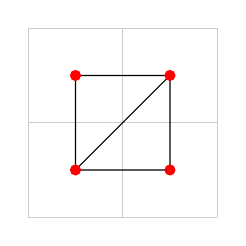
\begin{tikzpicture}[scale=1.2]
	    \draw[black!20] (0,0) grid (2,2);
	    \draw (0.5,0.5) rectangle (1.5,1.5) -- (0.5,0.5);
	    \filldraw[red] (0.5,0.5) circle [radius=1.5pt]
		      (1.5,0.5) circle [radius=1.5pt]
		      (0.5,1.5) circle [radius=1.5pt]
		      (1.5,1.5) circle [radius=1.5pt];
	\end{tikzpicture}
    \end{subfigure}
    \caption{Gitterwahl für die Diskretisierung: links $2\times 2$ Pixel, rechts zugehöriges Gitter. Die Knotenpunkte liegen in der Mitte der zugehörigen Pixel.}
    \label{fig:grid}
\end{figure}

Für einfache lineare Lagrange Basisfunktionen können die Pixelwerte des Bildes auf diese Weise eins zu eins in der diskreten Funktion als DOF-Vektor repräsentiert werden.
Insbesondere besitzt der entsprechende DOF-Vektor die selbe Anzahl Freiheitsgrade wie das ursprüngliche Bild.

Eine Gitterverfeinerung von $\scr T_0$ wird gemäß Abbildung \ref{fig:refine} durch Dreiecksviertelung durchgeführt und wir bezeichnen die entstehenden Triangulierungen mit $\scr T_q$, $q \in \N$.

\begin{figure}[ht]
    \centering
    \begin{subfigure}{0.4\textwidth}
	\centering
	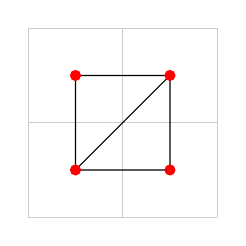
\begin{tikzpicture}[scale=1.2]
	    \draw[black!20] (0,0) grid (2,2);
	    \draw (0.5,0.5) rectangle (1.5,1.5) -- (0.5,0.5);
	    \filldraw[red] (0.5,0.5) circle [radius=1.5pt]
		      (1.5,0.5) circle [radius=1.5pt]
		      (0.5,1.5) circle [radius=1.5pt]
		      (1.5,1.5) circle [radius=1.5pt];
	\end{tikzpicture}
	\caption{$q = 0$}
    \end{subfigure}%
    \begin{subfigure}{0.4\textwidth}
	\centering
	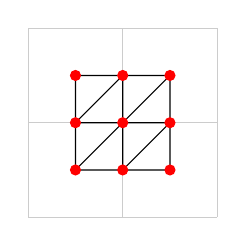
\begin{tikzpicture}[scale=1.2]
	    \draw[black!20] (0,0) grid (2,2);
	    \draw (0.5,0.5) rectangle (1.5,1.5) -- (0.5,0.5);
	    \draw (0.5,1) -- (1,1.5) -- (1,1) -- cycle;
	    \draw (1,0.5) -- (1.5,1) -- (1,1) -- cycle;
	    \filldraw[red] (0.5,0.5) circle [radius=1.5pt]
		      (1.5,0.5) circle [radius=1.5pt]
		      (0.5,1.5) circle [radius=1.5pt]
		      (1.5,1.5) circle [radius=1.5pt]
		      (0.5,1) circle [radius=1.5pt]
		      (1,0.5) circle [radius=1.5pt]
		      (1,1) circle [radius=1.5pt]
		      (1,1.5) circle [radius=1.5pt]
		      (1.5,1) circle [radius=1.5pt]
		      (1.5,1.5) circle [radius=1.5pt];
	\end{tikzpicture}
	\caption{$q = 1$}
    \end{subfigure}%
    \caption{Gitterverfeinerung}
    \label{fig:refine}
\end{figure}

Die diskreten Funktionen auf der Triangulierung $\scr T_q$ sind teilweise durch unterschiedliche Basisfunktionen repräsentiert, wie im Folgenden erläutert.
\begin{itemize}
    \item
	Mit Blick auf die entsprechende partielle Differentialgleichung \eqref{eq:pde_u} wählen wir $u \in \P_1(\scr T_q)$, d.h. $u$ ist durch lineare Lagrange-Basisfunktionen repräsentiert.
	Gleichermaßen setzen wir $n \in \P_1^d(\scr T_q)$ an.

	Für $n$ liesen sich allgemeinere, $H^{\mathrm{div}}$-konforme Basisfunktionen wählen (siehe \cite[§3]{logg2012automated} für eine Auswahl).
        %Diese standen jedoch in \texttt{dune-fem} nicht zur Verfügung, weshalb gewöhnliche lineare Lagrange-Basisfunktionen für $n$ gewählt wurden.
    \item
	Für $p$ und $m$ wählen wir konstante, diskontinuierliche Basisfunktionen, d.h. $p, m \in \D_0(\scr T_q)$.
       	Begründung hierfür sind die elementweise konstanten Ausdrücke $\nabla u$ und $\nabla \cdot n$ im $p$-Update und die Nebenbedingung $|p| - m\cdot p$.
    \item
	Natürlicherweise ergeben sich dann $\lambda_1, \lambda_2$ konstant diskontinuierlich aus den Lagrange"=Updates.
    \item
	Unklar ist die Wahl für $\lambda_4$: in jedem Fall wäre eine Projektion nötig, da $n$ und $m$ verschieden repräsentiert sind.
	Wir wählen $\lambda_4$ ebenfalls konstant diskontinuierlich.
\end{itemize}
Diese Wahlen wurden getroffen, um die entstehenden Fehler bei den nötigen Projektionen zwischen verschiedenen diskreten Räumen zu minimieren.
Die nötigen Projektionen befinden sich bei dieser Wahl nur im $m$- und im $\lambda_4$-Update.








\section{Implementierung}


Die Implementierung fand in der Programmiersprache C++ statt.
Wie bereits erwähnt, wurden die Dune-Module \texttt{dune-fem} und \texttt{dune-acfem} verwendet.
%Verwendet wurden die GPLv2-lizenzierte, C++ „Distributed and Unified Numerics Environment“ Dune\footnote{\url{https://dune-project.org}} samt Core-Modulen, sowie den Modulen \texttt{dune-fem} und \texttt{dune-acfem}.
Dabei ist \texttt{dune-fem} für die Finite Elemente Diskretisierung zuständig und \texttt{dune-acfem} bietet darauf aufbauend eine zusätzliche komfortable Abstraktionsebene.

Für die Visualisierung wurde das BSD-lizenzierte Toolkit VTK \cite{schroeder2004visualization} genutzt, das verschiedene Möglichkeiten zur Repräsentierung und Visualisierung von Daten und Bildern bietet.

Ohne die Implementierung im Detail zu beschreiben, soll an dieser Stelle ein kurzer Überblick über die wesentlichen Teile des in dieser Arbeit entstandenen Quellcodes gegeben werden.
Hinweise zur Installation oder konkreten Verwendung finden sich in der beiliegenden \texttt{README.md}.
Es sei angemerkt, dass Performance nicht das Hauptaugenmerk während der Implementierung darstellte.

\begin{description}
    \item[\texttt{build/src/eeinpaint\{,_gui\}}]
	Die beiden ausführbaren Dateien führen den Inpainting-Algorithmus aus.
 	Das Programm \path{build/src/eeinpaint_gui} startet den Algorithmus in einem separaten Thread, um eine in Echtzeit aktualisierte graphische Oberfläche anzuzeigen, auf der die Entwicklung von $u$, sowie verschiedene hilfreiche Werte beobachtet werden können.
	Dagegen ist \path{build/src/eeinpaint} rein kommandozeilenbasiert und generiert Log-Daten in Form von Tab"=separierten Werten, sowie das Endresultat für $u$ als VTK Unstructured Grid (Endungen \texttt{.pvtu} und \texttt{.vtu}) im Verzeichnis \texttt{output}.

	Parameter können entweder in \path{data/parameter} eingestellt werden (siehe unten), oder direkt bei Programmaufruf übergeben werden.
    \item[\texttt{src/algorithm_\{base,live,logging\}.hh}]
	Das Herzstück der Implementierung findet sich in \path{algorithm_base.hh}: die Klasse \Code{AlgorithmBase} definiert Methoden für die Teilschritte des Algorithmus, sowie eine Methode \Code{run()}, welche den Algorithmus durchführt.

	Um die Ergebnisse auszugeben, oder zusätzliche Daten während des Algorithmus zu erheben, wird die Klasse durch \Code{AlgorithmLive} und \Code{AlgorithmLogging} entsprechend erweitert.
    \item[\texttt{src/main\{,_gui\}.cc}]
	Dies sind die Programmeinstiegspunkte der beiden generierten ausführbaren Dateien \path{src/eeinpaint} und \path{src/eeinpaint_gui}.
	Hier wird die Bilddatei für $u^0$ gelesen, das Gitter erzeugt und unter Umständen verfeinert, um anschließend den entsprechenden Algorithmus aufzurufen.
   \item[\texttt{data/input\{,_mask\}.png}]
	Die Datei \path{data/input.png} wird in Graustufen gelesen und repräsentiert $u^0$.
	Dazu wird eine Inpainting-Maske aus \path{data/input_mask.png} gelesen, welche den Inpaintingbereich angibt: schwarz für $\Omega \setminus D$, weiß für $D$.
    \item[\texttt{data/parameter}]
	Hier werden die nötigen Parameter für den Algorithmus eingestellt.
	Folgende Parameter sind wesentlich.
	\begin{description}
	    \item[\texttt{eeinpaint.\{alpha,beta,eta\}}]
		Parameter $\alpha$, $\beta$, $\gamma$ in der ursprünglichen Inpaintingenergie,
	    \item[\texttt{eeinpaint.\{r1,r2,r4\}}]
		Penalty-Parameter für das Augmented Lagrange Verfahren,
	    \item[\texttt{eeinpaint.refinements}]
		Anzahl initialer Verfeinerungen des Gitters,
	    \item[\texttt{eeinpaint.maxOuterIterations}]
		Abbruchkriterium für die Anzahl Schleifendurchläufe in Algorithmus \ref{alg:ee}, entspricht $\kmax$ in \eqref{eq:stopmax}.
	\end{description}
    \item[\texttt{tools/runjob.sh}]
	Dies ist ein Wrapper für \path{build/src/eeinpaint}, um mehrere Jobs parallel laufen lassen zu können.
	Die erzeugten Dateien werden in ein Unterverzeichnis im Ordner \path{output} abgelegt, um keine Konflikte zu erzeugen.
    \item[\texttt{tools/vtkconvert.sh}]
	Dieses Skript rendert VTK Unstructured Grid Dateien (Endung \texttt{.pvtu} und \text{.vtu}) mit Wertebereich $[0,1]$ durch Parallelprojektion zu Graustufen-PNG-Bilder.
\end{description}


Angedacht, aber nicht umgesetzt sind folgende Ideen.
\begin{itemize}
    \item
	Eine adaptive Verfeinerung des Gitters wäre angebracht und könnte die Stärken einer Finiten Elemente Implementierung zum Vorschein bringen.
	Zur Bewertung könnte $|\nabla u|$ dienen, um scharfe Kanten besser auflösen zu können und in weniger interessanten Bereichen des Bildes nicht zu viel Rechenzeit zu verschwenden.
    \item
	Einige Schritte des Algorithmus \ref{alg:ee} sind unabhängig voneinander und könnten parallel arbeiten.
	Abgesehen von den offensichtlich unabhängigen Lagrange-Updates, ist beispielsweise die PDE für $u$ nicht abhängig von $n$ oder $\lambda_4$ im Schritt zuvor, was bedeutet, dass die beiden kostspieligen PDEs parallel berechnet werden könnten.
\end{itemize}

Um einen Teil unserer Implementierung zu testen, wurde der Algorithmus \ref{alg:ee} auch separat für reines TV-Inpainting implementiert: dabei wurden alle Variablen und Parameter ausgelassen, welche nur für den Krümmungsanteil in der Inpainting-Energie \eqref{eq:energy_splitted} benötigt werden, siehe Algorithmus \ref{alg:tv}.

\begin{algorithm}[TV Inpainting] \label{alg:tv}
    \Input{$\Omega \subset \R^2$, $u^0: \Omega \setminus D \to \R$, $\alpha, \eta \in \R_{> 0}$, $r_2 \in \R_{>0}$} \\
    \Output{$(u^k: \Omega \to \R)_{k\in\N}$}
    \begin{algorithmic}
	\State{$p^0, \lambda_2^0 \gets 0$}
	\For{$k = 0, 1, \dotsc$}
	    \State{$\Big.u^{k+1} \gets \solve{u} 0 = \int_\Omega (r_2 \nabla u - r_2 p^k - \lambda_2^k) \cdot \nabla \phi + \eta \int_{\Omega\setminus D} (u - u^0) \phi$}
	    \State{$\Big.p^{k+1} \gets \max\big\{0, 1 - \frac{\alpha}{q^k}\big\}q^k$, wobei $q^k = \nabla u^{k+1} - \frac{\lambda_2^k}{r_2}$}
	    \State{$\Big.\lambda_2^{k+1} \gets \lambda_2^k + r_2(p^{k+1} - \nabla u^{k+1})$}
	\EndFor
    \end{algorithmic}
    \begin{note}
	Dieser Algorithmus unterscheidet sich von \ref{alg:ee} mit der Wahl $\beta = 0$, da die Variablen $n, m, \lambda_1, \lambda_4$ nicht mehr auftreten und somit Fehler, die durch Projektionen entstehen, keine Auswirkungen mehr haben.
    \end{note}
\end{algorithm}


\section{Synthetische Tests und Parameterstudie}

Beim Testen unserer Implementierung von Algorithmus \ref{alg:ee} haben sich Auffälligkeiten im Zusammenhang der Parameterwahlen $r_1, r_2, r_4$ ergeben, die wir mit Hilfe einer Parameterstudie untersucht haben.

Das in den folgenden Tests genutzte, synthetische $u^0$ befindet sich in Abbildung \ref{fig:sample} links.

\begin{figure}[ht]
    \begin{subfigure}{0.33\textwidth}
	\centering
	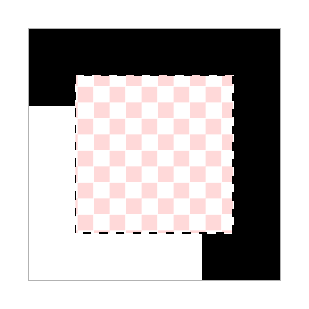
\begin{tikzpicture}[scale=0.1]
	    \filldraw[black] (0,0) rectangle (32,32);
	    \filldraw[white] (0,0) rectangle (22,22);
	    \filldraw[white] (6,6) rectangle (26,26);
	    \draw[missing] (6,6) rectangle (26,26);
	    \draw[black!30] (0,0) rectangle (32,32);
	\end{tikzpicture}
    \end{subfigure}%
    \begin{subfigure}{0.33\textwidth}
	\centering
	
\begin{tikzpicture}[scale=0.1]
	    \filldraw[black] (0,0) rectangle (32,32);
	    \filldraw[white] (0,0) -- (22,0) -- (22,6) -- (6,22) -- (0,22) -- cycle;
	    \draw[black!30] (0,0) rectangle (32,32);
	\end{tikzpicture}
    \end{subfigure}%
    \begin{subfigure}{0.33\textwidth}
	\centering
	
\begin{tikzpicture}[scale=0.1]
	    \clip (0,0) rectangle (32,32);
	    \filldraw[black] (0,0) rectangle (32,32);
	    \filldraw[white,rounded corners=50] (-22,-22) rectangle (22,22);
	    \draw[black!30] (0,0) rectangle (32,32);
	\end{tikzpicture}
    \end{subfigure}%
    \caption{In den numerischen Tests vorgegebenes $32\times 32$ Pixel Inpaintingproblem (links) zusammen mit theoretisch wünschenswertem TV-Inpainting (mittig) und Elastica-Inpainting (rechts)}
    \label{fig:sample}
\end{figure}

Für TV-Inpainting erwarten wir als Lösung eine diagonale, gerade verlaufende Schwarz-Weiß-Kante, während Elastica-Inpainting eine (je nach Wahl von $\alpha, \beta$) gekrümmte Kante hervorbringen sollte.

Zwei Abbruchkriterien wurden implementiert:
\begin{itemize}
    \item
	Eine maximale Anzahl Iterationen wurde erreicht:
	\begin{math}[numbered] \label{eq:stopmax}
	    k > \kmax.
	\end{math}
    \item
	Die Summe der $L^2$-Fehler der Nebenbedingungen ist hinreichend klein:
	\begin{math}[numbered] \label{eq:stopres}
	    \underbrace{\||p^k| - m^k \cdot p^k\|_{L^2}}_{=:R_{mp}^k} + \underbrace{\|p^k - \nabla u^k\|_{L^2}}_{=:R_{pu}^k} + \underbrace{\|n^k - m^k\|_{L^2}}_{=:R_{nm}^k} < \epsilon_R.
	\end{math}
	Dieses Abbruchkriterium orientiert sich ebenfalls an \cite{tai2011fast}.
	Es sei angemerkt, dass sich $n \in \P_k^2(\scr T_q)$ und $m \in \D_k^2(\scr T_q)$ bei unserer Implementierung in verschiedenen diskreten Räumen befinden und $\|n^k - m^k\|_{L^2} = 0$ nur dann erfüllt sein kann, wenn $n = m$ konstant sind.
\end{itemize}

\DeclareDocumentCommand{\Limg}{}{\scr L_{\mathrm{img}}}
\DeclareDocumentCommand{\Ldat}{}{\scr L_{\mathrm{dat}}}
\DeclareDocumentCommand{\Lconstr}{}{\scr L_{\mathrm{constr}}}
\DeclareDocumentCommand{\Ltotal}{}{\scr L_{\mathrm{total}}}

Wir protokollieren unter anderem
die $L^2$-Abstände aufeinanderfolgender Itererierten, obige Lagrange"=Update Residuen $R_{mp}^k$, $R_{pu}^k$, $R_{nm}^k$, sowie
die numerischen Energien
\begin{math}
    \Limg^k &:= \int_\Omega \big(\alpha + \beta (\nabla \cdot n^k)^2\big)|p^k|, \\
    \Ldat^k &:= \frac{\eta}{2} \int_{\Omega\setminus D} |u^k - u^0|^2, \\
    \Lconstr^k &:=
	r_1 \int_\Omega (|p^k| - m^k\cdot p^k) + \int_\Omega \lambda_1 (|p^k| - m^k \cdot p^k) \\
	&\quad + \frac{r_2}{2} \int_\Omega |p^k - \nabla u^k|^2 + \int_\Omega \lambda_2 \cdot (p^k - \nabla u^k) \\
	&\quad + \frac{r_4}{2} \int_\Omega |n^k - m^k|^2 + \int_\Omega \lambda_4 \cdot (n^k - m^k), \\
    \Ltotal^k &:= \Limg^k + \Ldat^k + \Lconstr^k.
\end{math}


Es sei angemerkt, dass die im Folgenden gezeigten Bildresultate in den numerischen Tests mit Hilfe des obigen Skripts \path{tools/vtkcontvert.sh} aus der diskreten Funktion $u$ auf dem Finite Elemente Gitter erstellt wurde.
Dabei rendert VTK die Funktion entsprechend der linearen Basisfunktionen in ein Graustufenbild von 5-facher Größe des Gitters.
Die Bilder suggerieren daher teilweise eine höhere Auflösung, als tatsächlich vorhanden.


%\begin{math}
%    \|u^k - u^{k-1}\|,
%    \|p^k - p^{k-1}\|,
%    \|m^k - m^{k-1}\|,
%    \|n^k - n^{k-1}\|,
%    \|\lambda_1^k - \lambda_1^{k-1}\|,
%    \|\lambda_2^k - \lambda_2^{k-1}\|,
%    \|\lambda_4^k - \lambda_4^{k-1}\|.
%\end{math}

\subsection*{TV-Inpainting}

Wir testen nun den TV-Inpainting-Algorithmus \ref{alg:tv} und führen eine kleine Parameterstudie für $r_2$ durch.
Hierfür wählen wir $\alpha = 1$ und $\eta = 1000$, während wir $r_2 \in \Set{10^k}_{k=-2}^4$ variieren.
Als Abbruchkriterium wurde \eqref{eq:stopmax} mit $\kmax = 5000$ gewählt.

\DeclareDocumentCommand{\Etv}{}{E_{\mathrm{tv}}}

Die Inpainting-Energie aus \eqref{eq:energy_ee} ist hier von der Form
\begin{math}
    \Etv[u] = \int_\Omega \alpha |\nabla u| + \frac{\eta}{2} \int_{\Omega\setminus D} |u - u^0|^2.
\end{math}
Da wir für $u$ lineare Basisfunktionen angesetzt haben, lässt sich $E_{\mathrm{tv}}[u]$ ohne weiteres numerisch auswerten.
\begin{figure}[ht]
    \begin{subfigure}{0.4\textwidth}
	\centering
	\begin{tikzpicture}
	    \begin{semilogxaxis}[width=7cm,xlabel=$k$,restrict y to domain=260:268,each nth point={5}]
		%\addplot table [x=k,y=dataEnergy] {refinements=0_alpha=1e0_r2=1e-2/output.dat};
		%\addplot table [x=k,y=tv] {refinements=0_alpha=1e0_r2=1e-2/output.dat};
		\addplot table [x=k,y expr=\thisrow{tv}+\thisrow{dataEnergy}] {data/tvr2/refinements=0_alpha=1e0_r2=1e-2/output.dat};
		\addplot table [x=k,y expr=\thisrow{tv}+\thisrow{dataEnergy}] {data/tvr2/refinements=0_alpha=1e0_r2=1e-1/output.dat};
		\addplot table [x=k,y expr=\thisrow{tv}+\thisrow{dataEnergy}] {data/tvr2/refinements=0_alpha=1e0_r2=1e0/output.dat};
		\addplot table [x=k,y expr=\thisrow{tv}+\thisrow{dataEnergy}] {data/tvr2/refinements=0_alpha=1e0_r2=1e1/output.dat};
		\addplot table [x=k,y expr=\thisrow{tv}+\thisrow{dataEnergy}] {data/tvr2/refinements=0_alpha=1e0_r2=1e2/output.dat};
		\addplot table [x=k,y expr=\thisrow{tv}+\thisrow{dataEnergy}] {data/tvr2/refinements=0_alpha=1e0_r2=1e3/output.dat};
		\addplot table [x=k,y expr=\thisrow{tv}+\thisrow{dataEnergy}] {data/tvr2/refinements=0_alpha=1e0_r2=1e4/output.dat};
	    \end{semilogxaxis}
	\end{tikzpicture}
	\caption{$E_{\mathrm{tv}}[u^k]$ für verschiedene $r_2$.}
	\label{fig:num_tvr2_etv}
    \end{subfigure}
    \begin{subfigure}{0.6\textwidth}
	\centering
%\pgfplotscreateplotcyclelist{mycolor}{
%    {Set2-8-1},
%    {Set2-8-2},
%    {Set2-8-3},
%    {Set2-8-4},
%    {Set2-8-5},
%    {Set2-8-6},
%    {Set2-8-7},
%    {Set2-8-8}
%}
	\begin{tikzpicture}
	    \begin{loglogaxis}[width=7cm,xlabel=$k$,each nth point={5}]
		%\addplot table [x=k,y=dataEnergy] {refinements=0_alpha=1e0_r2=1e-2/output.dat};
		%\addplot table [x=k,y=tv] {refinements=0_alpha=1e0_r2=1e-2/output.dat};
		\addplot table [x=k,y=puConstr] {data/tvr2/refinements=0_alpha=1e0_r2=1e-2/output.dat};
		\addplot table [x=k,y=puConstr] {data/tvr2/refinements=0_alpha=1e0_r2=1e-1/output.dat};
		\addplot table [x=k,y=puConstr] {data/tvr2/refinements=0_alpha=1e0_r2=1e0/output.dat};
		\addplot table [x=k,y=puConstr] {data/tvr2/refinements=0_alpha=1e0_r2=1e1/output.dat};
		\addplot table [x=k,y=puConstr] {data/tvr2/refinements=0_alpha=1e0_r2=1e2/output.dat};
		\addplot table [x=k,y=puConstr] {data/tvr2/refinements=0_alpha=1e0_r2=1e3/output.dat};
		\addplot table [x=k,y=puConstr] {data/tvr2/refinements=0_alpha=1e0_r2=1e4/output.dat};
		\legend{
		  $r_2=10^{-2}$,
		  $r_2=10^{-1}$,
		  $r_2=10^0$,
		  $r_2=10^1$,
		  $r_2=10^2$,
		  $r_2=10^3$,
		  $r_2=10^4$,
		}
	    \end{loglogaxis}
	\end{tikzpicture}
	\caption{$R_{pu} = \|p - \nabla u\|_{L^2}$ für verschiedene $r_2$. \hspace{2cm} \mbox{}}
	\label{fig:num_tvr2_pu}
    \end{subfigure}
    \caption{TV-Inpainting}
\end{figure}

In Abbildung \ref{fig:num_tvr2_etv} sehen wir, dass die Energie $\Etv$ für alle Parameterwahlen $r_2$ annähernd gegen den selben Wert konvergiert.
Das beste Konvergenzverhalten ist für $r_2 = 10$ zu beobachten.
Für $r_2 \ge 10$ wird die Nebenbedingung $p = \nabla u$ wie erwartet durchgehend besser eingehalten (siehe Abbildung \ref{fig:num_tvr2_pu}) auf Kosten einer zu Beginn sehr hohen Energie $\Etv$.

Im Endergebnis für $k = 5000$ unterscheidet sich nur der Fall $r_2 = 10^4$ mit der höchsten Energie noch optisch von den restlichen Ergebnissen, wie exemplarisch in Abbildung \ref{fig:num_tvr2_png} zu sehen.

\begin{figure}[ht]
    \centering
    \begin{subfigure}{0.2\textwidth}
	\centering
	\myincludegraphics[width=0.8\textwidth]{data/tvr2/refinements=0_alpha=1e0_r2=1e-2/vtk.png}
	\caption{$r_2=10^{-2}$}
    \end{subfigure}%
    \begin{subfigure}{0.2\textwidth}
	\centering
	\myincludegraphics[width=0.8\textwidth]{data/tvr2/refinements=0_alpha=1e0_r2=1e2/vtk.png}
	\caption{$r_2=10^{1}$}
    \end{subfigure}%
    \begin{subfigure}{0.2\textwidth}
	\centering
	\myincludegraphics[width=0.8\textwidth]{data/tvr2/refinements=0_alpha=1e0_r2=1e4/vtk.png}
	\caption{$r_2=10^{4}$}
    \end{subfigure}%
    \caption{Inpaintingresultate für verschiedene $r_2$.}
    \label{fig:num_tvr2_png}
\end{figure}

%Für $r_2 \le 1$ ist die Energie zu Beginn relativ niedrig, erfährt jedoch erst einen deutlichen Abfall nachdem die Nebenbedingungen zu einem gewissen Grad eingehalten wurden.


% TODO: echte tv energie, vs numerische mit p


Anzumerken ist in Abbildung \ref{fig:num_tvr2_png} die Breite der diagonalen Kante, sowie die beiden kleinen Auswüchse an den jeweiligen Enden dieser.
Beides reduziert sich durch globale Verfeinerung des Gitters, wie in Abbildung \ref{fig:num_tvrefine_png} zu sehen.
Beide Phänomene gehen auch für ein um 90° gedrehtes Eingabebild deutlich zurück, wie in Abbildung \ref{fig:num_tvgrid} zu sehen.
Dies lässt sich durch die Gitterstruktur in Abbildung \ref{fig:grid} erklären: für das rotierte Eingabebild ist die diagonale Schwarz-Weiß Kante des Inpaintingresultats nun an den diagonalen Dreieckskanten im Gitter ausgerichtet.

\begin{figure}[ht]
    \centering
    \begin{subfigure}{0.2\textwidth}
	\centering
	\myincludegraphics[width=0.8\textwidth]{data/tvgrid/vtk.png}
	\caption{$q=0$, rotiert}
	\label{fig:num_tvgrid}
    \end{subfigure}%
    \begin{subfigure}{0.2\textwidth}
	\centering
	\myincludegraphics[width=0.8\textwidth]{data/tvrefine/refinements=0_alpha=1e0_r2=1e1/vtk.png}
	\caption{$q=0$}
    \end{subfigure}%
    \begin{subfigure}{0.2\textwidth}
	\centering
	\myincludegraphics[width=0.8\textwidth]{data/tvrefine/refinements=1_alpha=1e0_r2=1e1/vtk.png}
	\caption{$q=1$}
    \end{subfigure}%
    \begin{subfigure}{0.2\textwidth}
	\centering
	\myincludegraphics[width=0.8\textwidth]{data/tvrefine/refinements=4_alpha=1e0_r2=1e1/vtk.png}
	\caption{$q=4$}
    \end{subfigure}%
    \caption{Auswirkungen des Gitters auf das Inpainting-Resultat für $r_2=10^1$.}
    \label{fig:num_tvrefine_png}
\end{figure}



%\begin{figure}[ht]
%    \centering
%    \begin{tikzpicture}
%	\begin{semilogxaxis}[width=10cm,height=6cm,xlabel=$k$,ylabel={$E_{\mathrm{tv}}[u^k]$}]
%	    %\addplot table [x=k,y=dataEnergy] {refinements=0_alpha=1e0_r2=1e-2/output.dat};
%	    %\addplot table [x=k,y=tv] {refinements=0_alpha=1e0_r2=1e-2/output.dat};
%	    \addplot table [x=k,y expr=\thisrow{tv}] {data/tvrefine/refinements=0_alpha=1e0_r2=1e1/output.dat};
%	    \addplot table [x=k,y expr=\thisrow{tv}] {data/tvrefine/refinements=1_alpha=1e0_r2=1e1/output.dat};
%	    \addplot table [x=k,y expr=\thisrow{tv}] {data/tvrefine/refinements=2_alpha=1e0_r2=1e1/output.dat};
%	    \addplot table [x=k,y expr=\thisrow{tv}] {data/tvrefine/refinements=3_alpha=1e0_r2=1e1/output.dat};
%	    \addplot table [x=k,y expr=\thisrow{tv}] {data/tvrefine/refinements=4_alpha=1e0_r2=1e1/output.dat};
%	    \legend{
%	      $q=0$,
%	      $q=1$,
%	      $q=2$,
%	      $q=3$,
%	      $q=4$,
%	    }
%	\end{semilogxaxis}
%    \end{tikzpicture}
%    \caption{Totale Variation bei unterschiedlicher globaler Verfeinerung.}
%    \label{fig:num_tvrefine_tv}
%\end{figure}


\subsection*{Euler Elastica Inpainting}

Wenden wir uns nun Algorithmus \ref{alg:ee} zu.
Auch hier wünschen wir uns numerisch eine Konvergenz des Algorithmus und möglichst von den Penalty-Parametern $r_1, r_2, r_4$ unabhängige Endresultate.
Wir fixieren zunächst $\eta = 1000$ und untersuchen dies für die Wahlen $\alpha = 1, \beta = 1000$, sowie $\alpha = 1000$ und $\beta = 1$.
Dabei variieren wir jeweils
\begin{math}[numbered] \label{eq:num_param}
    r_1 \in \Set{10^0, 10^1, 10^2, 10^3, 10^4}, \qquad
    r_2, r_4 \in \Set{10^0, 10^2, 10^4}.
\end{math}
Wir erwarten aufgrund der Modifikation in \eqref{eq:energy_al} (die Verwendung von $L^1$-Penalizing statt $L^2$-Penalizing für $|p| = m\cdot p$)  und wählen daher eine feinere Auflösung für $r_1$.
%gewählt, da die Modifikation in \eqref{eq:energy_al} (die Verwendung von $L^1$-Penalizing statt $L^2$-Penalizing) höchstwahrscheinlich starke Auswirkungen auf die Größenordnung von $r_1$ hat.
Als Abbruchkriterium wird an dieser Stelle \eqref{eq:stopmax} gewählt mit $\kmax = 50000$.

\begin{figure}[ht]
    \begin{subfigure}{0.5\textwidth}
	\centering
	\begin{tikzpicture}
	    \begin{loglogaxis}[width=0.9\textwidth,height=6cm,xlabel=$k$,ylabel={$\|u_k - u_{k-1}\|_{L^2}$},legend pos=south west,each nth point={3}]
		\addplot table [x=k,y=uDist] {data/eeparam/refinements=0_alpha=1e0_beta=1e3_r1=1e0_r2=1e4_r4=1e4/output.dat};
		\addplot table [x=k,y=uDist] {data/eeparam/refinements=0_alpha=1e0_beta=1e3_r1=1e1_r2=1e4_r4=1e4/output.dat};
		\addplot table [x=k,y=uDist] {data/eeparam/refinements=0_alpha=1e0_beta=1e3_r1=1e2_r2=1e4_r4=1e4/output.dat};
		\legend{
		  $r_1 = 1$,
		  $r_1 = 10$,
		  $r_1 = 100$,
		}
	    \end{loglogaxis}
	\end{tikzpicture}
	\caption{$\alpha = 1$, $\beta = 1000$.}
	\label{fig:num_eeparam1_conv}
    \end{subfigure}%
    \begin{subfigure}{0.5\textwidth}
	\centering
	\begin{tikzpicture}
	    \begin{loglogaxis}[width=0.9\textwidth,height=6cm,xlabel=$k$,ylabel={$\|u_k - u_{k-1}\|_{L^2}$},legend pos=south west,each nth point={3}]
		\addplot table [x=k,y=uDist] {data/eeparam/refinements=0_alpha=1e3_beta=1e0_r1=1e0_r2=1e4_r4=1e4/output.dat};
		\addplot table [x=k,y=uDist] {data/eeparam/refinements=0_alpha=1e3_beta=1e0_r1=1e1_r2=1e4_r4=1e4/output.dat};
		\addplot table [x=k,y=uDist] {data/eeparam/refinements=0_alpha=1e3_beta=1e0_r1=1e2_r2=1e4_r4=1e4/output.dat};
		\legend{
		  $r_1 = 1$,
		  $r_1 = 10$,
		  $r_1 = 100$,
		}
	    \end{loglogaxis}
	\end{tikzpicture}
	\caption{$\alpha = 1000$, $\beta = 1$.}
	\label{fig:num_eeparam2_conv}
    \end{subfigure}%
    \caption{Elastica Inpainting: scheinbar konvergentes Verhalten für $r_2, r_4 = 10^4$.}
    \label{fig:num_eeparam_conv}
\end{figure}

Für hohe Parameter $r_2, r_4$ und niedriges $r_1$ zeigt der Algorithmus ein scheinbar konvergentes Verhalten (siehe Abbildung \ref{fig:num_eeparam_conv}) und man beobachtet Inpaintingergebnisse wie in den Abbildungen \ref{fig:num_eeparam_png} und \ref{fig:num_eeparam2_png}.
Diese Bilder zeigen für Elastica-Inpainting im Wesentlichen zu erwartende Ergebnisse: für größeres $\frac{\beta}{\alpha}$ erhält man ein bogenförmige Kante, während man für kleines $\frac{\beta}{\alpha}$ eine fast gerade Kante wie beim TV-Inpainting erhält.

Zu bemerken sind die in Abbildung \ref{fig:num_eeparam2_png} dunkleren Ergebnisse im Vergleich zu Abbildung \ref{fig:num_eeparam_png}.
Dies spricht dafür, dass sich durch die Veränderung von $\alpha$ und $\beta$ das Verhältnis zwischen Bildterm und Datenterm stark verändert hat und $\eta$ entsprechend angepasst werden sollte.

\begin{figure}[ht]
    \centering
    \begin{subfigure}{0.25\textwidth}
	\centering
	\myincludegraphics[width=0.7\textwidth]{data/eeparam/refinements=0_alpha=1e0_beta=1e3_r1=1e0_r2=1e4_r4=1e4/vtk.png}
	\caption{$r_1 = 1$}
    \end{subfigure}%
    \begin{subfigure}{0.25\textwidth}
	\centering
	\myincludegraphics[width=0.7\textwidth]{data/eeparam/refinements=0_alpha=1e0_beta=1e3_r1=1e1_r2=1e4_r4=1e4/vtk.png}
	\caption{$r_1 = 10$}
    \end{subfigure}%
    \begin{subfigure}{0.25\textwidth}
	\centering
	\myincludegraphics[width=0.7\textwidth]{data/eeparam/refinements=0_alpha=1e0_beta=1e3_r1=1e2_r2=1e4_r4=1e4/vtk.png}
	\caption{$r_1 = 100$}
    \end{subfigure}%
    \caption{Elastica Inpaintingresultate für $\alpha = 1$, $\beta = 1000$, $r_2, r_4 = 10^4$.}
    \label{fig:num_eeparam_png}
\end{figure}

\begin{figure}[ht]
    \centering
    \begin{subfigure}{0.25\textwidth}
	\centering
	\myincludegraphics[width=0.7\textwidth]{data/eeparam/refinements=0_alpha=1e3_beta=1e0_r1=1e0_r2=1e4_r4=1e4/vtk.png}
	\caption{$r_1 = 1$}
    \end{subfigure}%
    \begin{subfigure}{0.25\textwidth}
	\centering
	\myincludegraphics[width=0.7\textwidth]{data/eeparam/refinements=0_alpha=1e3_beta=1e0_r1=1e1_r2=1e4_r4=1e4/vtk.png}
	\caption{$r_1 = 10$}
    \end{subfigure}%
    \begin{subfigure}{0.25\textwidth}
	\centering
	\myincludegraphics[width=0.7\textwidth]{data/eeparam/refinements=0_alpha=1e3_beta=1e0_r1=1e2_r2=1e4_r4=1e4/vtk.png}
	\caption{$r_1 = 100$}
    \end{subfigure}%
    \caption{Elastica Inpaintingresultate für $\alpha = 1000$, $\beta = 1$, $r_2, r_4 = 10^4$.}
    \label{fig:num_eeparam2_png}
\end{figure}

Die Inpaintingresultate hängen leider vom Parameter $r_1$ ab und man beobachtet in den Abbildungen \ref{fig:num_eeparam_png} und \ref{fig:num_eeparam2_png} für höheres $r_1$ eine stärker nach außen gebogene Kante.

\begin{figure}[ht]
    \centering
    \begin{tikzpicture}
	\begin{loglogaxis}[width=10cm,height=6cm,xlabel=$k$,ylabel={$\|u_k - u_{k-1}\|_{L^2}$},each nth point={2}]
	    \addplot table [x=k,y=uDist] {data/eeparam/refinements=0_alpha=1e0_beta=1e3_r1=1e1_r2=1e2_r4=1e2/output.dat};
	    \addplot table [x=k,y=uDist] {data/eeparam/refinements=0_alpha=1e0_beta=1e3_r1=1e3_r2=1e4_r4=1e4/output.dat};
	    \legend{
	      {$r_1 = 10, r_2,r_4 = 100$},
	      {$r_1 = 1000, r_2,r_4 = 10000$},
	    }
	\end{loglogaxis}
    \end{tikzpicture}
    \caption{Elastica Inpainting: instabiles Verhalten für $\alpha = 1$, $\beta = 1000$.}
    \label{fig:num_eeparam_instab}
\end{figure}

Für größere $r_1$ oder kleinere $r_2, r_4$ zeigen sich Instabilitäten und man ist weit entfernt von Konvergenz (siehe exemplarisch Abbildung \ref{fig:num_eeparam_instab}).
Eine mögliche Erklärung hierfür ist das $L^1$-Penalizing in \eqref{eq:energy_al}: der $L^1$-Fehler überwiegt die $L^2$-Fehler für kleine Abweichungen erheblich und könnte zu aufschaukelnden Effekten führen.
Wird $r_1$ im Vergleich zu $r_2, r_4$ klein gehalten, ist dieses Phänomen nicht mehr spürbar.

Untersuchen wir nun den Fall $r_1 = 1$, $r_2, r_4 = 10^4$ der obigen Parameterstudie genauer.
In Abbildung \ref{fig:num_eeparam_energy} sehen wir $\scr L_{\mathrm{img}}^k$, $\scr L_{\mathrm{dat}}^k$, $\scr L_{\mathrm{constr}}$ und $\scr L_{\mathrm{total}}^k$ im Laufe des Algorithmus.

\begin{figure}[ht]
    \begin{subfigure}{0.5\textwidth}
	\centering
	\begin{tikzpicture}
	    \begin{semilogxaxis}[width=0.9\textwidth,xlabel=$k$,legend pos=north east,each nth point={4}]
		\addplot table [x=k,y=imageEnergy]  {data/eeparam/refinements=0_alpha=1e0_beta=1e3_r1=1e0_r2=1e4_r4=1e4/output.dat};
		\addplot table [x=k,y=dataEnergy]   {data/eeparam/refinements=0_alpha=1e0_beta=1e3_r1=1e0_r2=1e4_r4=1e4/output.dat};
		\addplot table [x=k,y=constrEnergy] {data/eeparam/refinements=0_alpha=1e0_beta=1e3_r1=1e0_r2=1e4_r4=1e4/output.dat};
		\addplot table [x=k,y=totalEnergy]  {data/eeparam/refinements=0_alpha=1e0_beta=1e3_r1=1e0_r2=1e4_r4=1e4/output.dat};
		\legend{
		    $\scr L_{\mathrm{img}}^k$,
		    $\scr L_{\mathrm{dat}}^k$,
		    $\scr L_{\mathrm{constr}}^k$,
		    $\scr L_{\mathrm{total}}^k$,
		}
	    \end{semilogxaxis}
	\end{tikzpicture}
	\caption{Numerische Energien.}
	\label{fig:num_eeparam_energy}
    \end{subfigure}%
    \begin{subfigure}{0.5\textwidth}
	\centering
	\begin{tikzpicture}
	    \begin{loglogaxis}[width=0.9\textwidth,xlabel=$k$,legend pos=north west,each nth point={3}]
		\addplot table [x=k,y=mpConstr] {data/eeparam/refinements=0_alpha=1e0_beta=1e3_r1=1e0_r2=1e4_r4=1e4/output.dat};
		\addplot table [x=k,y=puConstr] {data/eeparam/refinements=0_alpha=1e0_beta=1e3_r1=1e0_r2=1e4_r4=1e4/output.dat};
		\addplot table [x=k,y=nmConstr] {data/eeparam/refinements=0_alpha=1e0_beta=1e3_r1=1e0_r2=1e4_r4=1e4/output.dat};
		\legend{
		  $R_{mp}^k$,
		  $R_{pu}^k$,
		  $R_{nm}^k$,
		}
	    \end{loglogaxis}
	\end{tikzpicture}
	\caption{$L^2$-Fehler der Nebenbedingungen.}
	\label{fig:num_eeparam_constr}
    \end{subfigure}
    \caption{Elastica Inpainting mit $r_1 = 1$, $r_2, r_4 = 10^4$.}
\end{figure}

Auffällig ist das nicht-monotone Verhalten von $\scr L_{\mathrm{constr}}$.
Auch scheinen sich die Energien bis zum Schluss für $k = 50 000$ nicht stabilisiert zu haben: die Energien steigen, während $R_{mp}^k$ in Abbildung \ref{fig:num_eeparam_constr} deutlich sinkt (man beachte die logarithmischen Achsen).

Da die Nebenbedingung $|p| = m \cdot p$ als einzige den Einfluss des Krümmungsanteils der Elastica-Energie auf $u$ kontrolliert (siehe \eqref{eq:energy_splitted}), ist der Penalty-Parameter $r_1$ von wesentlicher Bedeutung.
Zudem sind die numerischen Energien wenig aussagekräftig, wenn diese wichtige Nebenbedingung kaum eingehalten wird.

Wir versuchen nun die Penalty-Parameter gemeinsam hochzuskalieren und setzen $r_1 = 1000$, $r_2, r_4 = 10^7$.
Als Abbruchkriterium kommt \eqref{eq:stopmax} zum Einsatz mit $\kmax = 2500$, während $\alpha = 1$, $\beta = 1000$ gewählt ist.

\begin{figure}[ht]
    \begin{subfigure}{0.5\textwidth}
	\centering
	\begin{tikzpicture}
	    \begin{semilogxaxis}[width=0.9\textwidth,xlabel=$k$,legend pos=south west]
		\addplot table [x=k,y=imageEnergy]  {data/eescale/output.dat};
		\addplot table [x=k,y=dataEnergy]   {data/eescale/output.dat};
		\addplot table [x=k,y=constrEnergy] {data/eescale/output.dat};
		\addplot table [x=k,y=totalEnergy]  {data/eescale/output.dat};
		\legend{
		    $\scr L_{\mathrm{img}}^k$,
		    $\scr L_{\mathrm{dat}}^k$,
		    $\scr L_{\mathrm{constr}}^k$,
		    $\scr L_{\mathrm{total}}^k$,
		}
	    \end{semilogxaxis}
	\end{tikzpicture}
	\caption{Numerische Energien.}
	\label{fig:num_eescale_energy}
    \end{subfigure}%
    \begin{subfigure}{0.5\textwidth}
	\centering
	\begin{tikzpicture}
	    \begin{loglogaxis}[width=0.9\textwidth,xlabel=$k$,legend pos=south west]
		\addplot table [x=k,y=mpConstr] {data/eescale/output.dat};
		\addplot table [x=k,y=puConstr] {data/eescale/output.dat};
		\addplot table [x=k,y=nmConstr] {data/eescale/output.dat};
		\legend{
		  $R_{mp}^k$,
		  $R_{pu}^k$,
		  $R_{nm}^k$,
		}
	    \end{loglogaxis}
	\end{tikzpicture}
	\caption{$L^2$-Fehler der Nebenbedingungen.}
	\label{fig:num_eescale_constr}
    \end{subfigure}
    \caption{Elastica Inpainting: Verhalten für hohe Penalty-Parameter}
    \label{fig:num_eescale}
\end{figure}

In Abbildung \ref{fig:num_eescale_energy} sehen wir, dass sich ab $k = 600$ ein fast stationärer Zustand der Energien eingestellt hat.
Die $L^2$-Fehler der Nebenbedingung $p = \nabla u$ und $|p| = m\cdot p$ in Abbildung \ref{fig:num_eescale_constr} fallen bei $k = 600$ dagegen stark ab, während $R_{nm}^k$ davon nicht derart betroffen ist.
Als Inpaintingresultat für $u$ erhält man ein fast konstantes, graues Bild.

Wir hatten gesehen, dass sich $m$ und $n$ in verschiedenen diskreten Räumen befinden: während $n$ durch linear stetige Basisfunktionen repräsentiert ist, sind es für $m$ konstante, diskontinuierliche.
Dies hat zur Folge, dass $R_{nm}^k = \|m-n\|_{L^2} = 0$ nur dann gelten kann, wenn $n$ und $m$ konstant sind.
Es wäre daher möglich, dass die hohe Wahl der Penalty-Parameter das Ergebnis unbrauchbar gemacht hat.




\section*{Denoising}


Wir wollen nun unseren Algorithmus zum Entrauschen von Bildern testen, d.h. wir geben $u^0$ auf ganz $\Omega$ vor und damit $D = \emptyset$.
Das Ursprungsbild $u^0$ hat die Größe $50\times 50$ Pixel und findet sich in Abbildung \ref{fig:num_denoise_orig}.
Wie in Kapitel \ref{chap:intro} besprochen, modelliert unser Bildmodel additives Gauß'sches Rauschen.
Wir simulieren daher in Abbildung \ref{fig:num_denoise_noise} Gauß'sches Rauschen gemäß \eqref{eq:gnoise} mit Varianz $\sigma^2 = 0.05$.
Außerdem treffen wir die Parameterwahlen $\alpha = 1$, $\beta = 1000$, $\eta = 800$, $r_1 = 20$, $r_2, r_4 = 10^{4}$ und wählen als Abbruchbedingung \eqref{eq:stopmax} mit $\kmax = 2500$.

\begin{figure}[ht]
    \centering
    \begin{subfigure}{0.25\textwidth}
	\centering
	\myincludegraphics[width=0.7\textwidth]{data/eedenoise/yinyang.png}
	\caption{Orginal}
	\label{fig:num_denoise_orig}
    \end{subfigure}%
    \begin{subfigure}{0.25\textwidth}
	\centering
	\myincludegraphics[width=0.7\textwidth]{data/eedenoise/yinyang_gaussian005.png}
	\caption{Verrauschtes Bild}
	\label{fig:num_denoise_noise}
    \end{subfigure}%
    \begin{subfigure}{0.25\textwidth}
	\centering
	\myincludegraphics[width=0.7\textwidth]{data/eedenoise/vtk.png}
	\caption{Denoising Resultat}
	\label{fig:num_denoise_result}
    \end{subfigure}%
    \caption{Elastica Denoisingresultate}
    \label{fig:num_denoise_png}
\end{figure}

Das Ergebnis in Abbildung \ref{fig:num_denoise_result} beseitigt das Gauß'sche Rauschen zufriedenstellend, während die Kanten dabei weitestgehend erhalten bleiben.
Allerdings verändern sich teilweise Formen im Bild gemäß des Elastica Bildmodells, wie man an den abgerundeten Spitzen der beiden Hälften erkennen kann.
Auch die Gitterstruktur hat, wie bereits beim TV-Inpainting erwähnt, Auswirkungen auf das Resultat: die beiden inneren Kreise sind leicht diagonal verzogen.


\section{Schlussbemerkungen}


Wir haben gesehen, dass das Elastica-Inpaintingmodell aus Definition
\ref{def:ee_inpainting} eine Verallgemeinerung des TV-Inpaintingmodells ist und im
Spezialfall $D = \emptyset$ auch zum Entrauschen von Bildern eingesetzt werden
kann.

Während das Elastica-Inpainting prinzipiell wünschenswerte Resultate liefert (siehe auch \cite{shen2002euler,tai2011fast} für entsprechende Bilder),
hat sich bei der Implementierung von Algorithmus \ref{alg:ee} im Kontext Finiter Elemente gezeigt, dass dieser sehr sensibel im Bezug auf die Penalty-Parameter ist.
Während für einige dieser Probleme die Ursache in der Finiten Elemente Diskretisierung liegen könnte, scheint das instabile Verhalten für hohes $r_1$ in Abbildung \ref{fig:num_eeparam_instab} dem $L^1$-Penalizing zu entstammen.
Auch die Autoren von \cite{tai2011fast}, auf dessen Algorithmus sich diese Arbeit gestützt hat, wählen für ihre Resultate ohne genauere Begründung jeweils sehr spezifische Penalty-Parameter.
Dies spricht dafür, dass die Sensibilität im Bezug auf $r_1, r_2, r_4$ dem Algorithmus inherent ist und nicht alleine von der Finiten Elemente Diskretisierung herrührt.

Ein Inpainting-Algorithmus, der nur für unbekannte, sehr spezielle Wahlen von Parametern schnelle und brauchbare Ergebnisse liefert, fordert zeitaufwändiges Optimieren der Parameterwahlen für jedes neue Eingabebild und ist daher generell nicht wünschenswert.
Trotzdem sind die in \cite{tai2011fast} und in dieser Arbeit benutzten Mittel („operator splitting“, „augmented lagrange“, „alternating direction“ Methode) brauchbare Werkzeuge, um dem Minimieren der Elastica-Inpaintingenergie aus \eqref{eq:energy_ee} entgegenzutreten.

Eine mögliche Idee um dem $L^1$-Penalizing zu entkommen wäre, das Minimierungsproblem aus Definition \ref{def:ee_inpainting} folgendermaßen zu splitten:
\begin{math}
    \min_{\substack{u \in C^2(\Omega,[0,1]) \\ s \in C^1(\Omega), n \in C^1(\Omega)^d}}
    &\scr E[s,n] = \int_\Omega \Big(\alpha + \beta(\nabla \cdot n)^2\Big)s + \frac{\eta}{2} \int_{\Omega \setminus D} |u - u_0|^2 \\
    &\quad \text{u.d.N.} \quad
	\nabla u \cdot n = s, \quad
	sn = \nabla u, \quad
	s \ge 0.
\end{math}
Man beachte, dass die Nebenbedingungen für $\nabla u \neq 0$ stets $n = \frac{\nabla u}{|\nabla u|}$ gewährleisten, während sie für $\nabla u = 0$ auch $s = 0$ einhalten und die Konvention aus Definition \ref{def:ee_inpainting} berücksichtigen.
Eine detailierte Analyse der Teilprobleme und Implementierung des zugehörigen „alternating direction“ Algorithmus ist im Rahmen dieser Arbeit nicht erfolgt.

Auch eine direkte Diskretisierung der Euler-Lagrange-Gleichung aus \cite{shen2002euler} wäre denkbar.
Um diese partielle Differentialgleichung vierter Ordnung im Kontext Finiter Elemente zu lösen, wären geeignete Methoden nötig, um bei der Assemblierung auch die zweiten Ableitungen der Basisfunktionen zu berücksichtigen.

Die relativ aktuellen Arbeiten \cite{brito2010fast,duan2013fast,hahn2011fast,tai2011fast,yashtini2015alternating} zeigen, dass schnelle numerische Lösungsverfahren für das Elastica-Bildmodell weiterhin gefragt sind und einer näheren Untersuchung bedürfen.


%Insgesamt beobachtet man für kleine $r_1$ sehr langsame Konvergenz und wenig aussagekräftige numerische Energien (da die wichtige Nebenbedingung nicht gut eingehalten wird), während großes $r_1$ zu Instabilitäten führt.

%
%\section{TEST}
%
%Sei nun $\alpha = 1000$ und $\beta = 1$ und variiere wie eben
%\begin{math}[numbered] \label{eq:num_param}
%    r_1 \in \Set{10^0, 10^1, 10^2, 10^3, 10^4}, \qquad
%    r_2, r_4 \in \Set{10^0, 10^2, 10^4}.
%\end{math}
%Als Abbruchkriterium wird wieder \eqref{eq:stopmax} mit $\kmax = 50000$ gewählt.
%
%\begin{figure}[ht]
%    \centering
%    \begin{tikzpicture}
%	\begin{loglogaxis}[width=9cm,height=6cm,xlabel=$k$,ylabel={$\|u_k - u_{k-1}\|_{L^2}$},each nth point={3}]
%	    \addplot table [x=k,y=uDist] {data/eeparam/refinements=0_alpha=1e3_beta=1e0_r1=1e0_r2=1e4_r4=1e4/output.dat};
%	    \addplot table [x=k,y=uDist] {data/eeparam/refinements=0_alpha=1e3_beta=1e0_r1=1e1_r2=1e4_r4=1e4/output.dat};
%	    %\addplot table [x=k,y=uDist] {data/eeparam/refinements=0_alpha=1e3_beta=1e0_r1=1e2_r2=1e4_r4=1e4/output.dat};
%	    \legend{
%	      $r_1 = 1$,
%	      $r_1 = 10$,
%	      $r_1 = 100$,
%	    }
%	\end{loglogaxis}
%    \end{tikzpicture}
%    \caption{Elastica Inpainting: konvergentes Verhalten für $r_2, r_4 = 10^4$.}
%    \label{fig:num_eeparam2_conv}
%\end{figure}
%
%\begin{figure}[ht]
%    \centering
%    \begin{tikzpicture}
%	\begin{loglogaxis}[width=10cm,height=6cm,xlabel=$k$,ylabel={$\|u_k - u_{k-1}\|_{L^2}$},each nth point={2}]
%	    \addplot table [x=k,y=uDist] {data/eeparam/refinements=0_alpha=1e3_beta=1e0_r1=1e1_r2=1e2_r4=1e2/output.dat};
%	    \addplot table [x=k,y=uDist] {data/eeparam/refinements=0_alpha=1e3_beta=1e0_r1=1e3_r2=1e4_r4=1e4/output.dat};
%	    \legend{
%	      {$r_1 = 10, r_2,r_4 = 100$},
%	      {$r_1 = 1000, r_2,r_4 = 10000$},
%	    }
%	\end{loglogaxis}
%    \end{tikzpicture}
%    \caption{Elastica Inpainting: instabiles Verhalten für größere $r_1$, bzw. kleinere $r_2, r_4$ als in Abbildung \ref{fig:num_eeparam_conv}.}
%    \label{fig:num_eeparam2_instab}
%\end{figure}
%
%Wir beobachten wieder konvergentes Verhalten für kleine $r_1$ und große $r_2, r_4$ (siehe Abbildung \ref{fig:num_eeparam2_conv}) und Instabilitäten sonst (siehe exemplarisch Abbildung \ref{fig:num_eeparam2_instab}).
%
%Für Parameterwahlen $r_1 = 1$, $r_2, r_4 = 10^4$ zeigen die Bilder in Abbildung \ref{fig:num_eeparam2_png} zu erwartende Ergebnisse ähnlich denen aus dem TV-Inpainting.
%Auch hier scheint der Parameter $r_1$ das Resultat zu beeinflussen.
%
%
%\begin{figure}[ht]
%    \centering
%    \begin{subfigure}{0.25\textwidth}
%	\centering
%	\myincludegraphics[width=0.7\textwidth]{data/eeparam/refinements=0_alpha=1e3_beta=1e0_r1=1e0_r2=1e4_r4=1e4/vtk.png}
%	\caption{$r_1 = 1$}
%    \end{subfigure}%
%    \begin{subfigure}{0.25\textwidth}
%	\centering
%	\myincludegraphics[width=0.7\textwidth]{data/eeparam/refinements=0_alpha=1e3_beta=1e0_r1=1e1_r2=1e4_r4=1e4/vtk.png}
%	\caption{$r_1 = 10$}
%    \end{subfigure}%
%    \begin{subfigure}{0.25\textwidth}
%	\centering
%	\myincludegraphics[width=0.7\textwidth]{data/eeparam/refinements=0_alpha=1e3_beta=1e0_r1=1e2_r2=1e4_r4=1e4/vtk.png}
%	\caption{$r_1 = 100$}
%    \end{subfigure}%
%    \caption{Elastica Inpaintingresultate für $r_2, r_4 = 10^4$.}
%    \label{fig:num_eeparam2_png}
%\end{figure}
%
%\begin{figure}[ht]
%    \begin{subfigure}{0.5\textwidth}
%	\centering
%	\begin{tikzpicture}
%	    \begin{semilogxaxis}[width=0.9\textwidth,xlabel=$k$,legend pos=south west,each nth point={4}]
%		\addplot table [x=k,y=imageEnergy]  {data/eeparam/refinements=0_alpha=1e3_beta=1e0_r1=1e2_r2=1e4_r4=1e4/output.dat};
%		\addplot table [x=k,y=dataEnergy]   {data/eeparam/refinements=0_alpha=1e3_beta=1e0_r1=1e2_r2=1e4_r4=1e4/output.dat};
%		\addplot table [x=k,y=constrEnergy] {data/eeparam/refinements=0_alpha=1e3_beta=1e0_r1=1e2_r2=1e4_r4=1e4/output.dat};
%		\addplot table [x=k,y=totalEnergy]  {data/eeparam/refinements=0_alpha=1e3_beta=1e0_r1=1e2_r2=1e4_r4=1e4/output.dat};
%		\legend{
%		    $\scr L_{\mathrm{img}}^k$,
%		    $\scr L_{\mathrm{dat}}^k$,
%		    $\scr L_{\mathrm{constr}}^k$,
%		    $\scr L_{\mathrm{total}}^k$,
%		}
%	    \end{semilogxaxis}
%	\end{tikzpicture}
%	\caption{Numerische Energien.}
%	\label{fig:num_eescale_energy}
%    \end{subfigure}%
%    \begin{subfigure}{0.5\textwidth}
%	\centering
%	\begin{tikzpicture}
%	    \begin{loglogaxis}[width=0.9\textwidth,xlabel=$k$,legend pos=north west,each nth point={3}]
%		\addplot table [x=k,y=mpConstr]   {data/eeparam/refinements=0_alpha=1e3_beta=1e0_r1=1e0_r2=1e4_r4=1e4/output.dat};
%		\addplot table [x=k,y=puConstr]   {data/eeparam/refinements=0_alpha=1e3_beta=1e0_r1=1e0_r2=1e4_r4=1e4/output.dat};
%		\addplot table [x=k,y=nmConstr]   {data/eeparam/refinements=0_alpha=1e3_beta=1e0_r1=1e0_r2=1e4_r4=1e4/output.dat};
%		\legend{
%		  $R_{mp}^k$,
%		  $R_{pu}^k$,
%		  $R_{nm}^k$,
%		}
%	    \end{loglogaxis}
%	\end{tikzpicture}
%	\caption{$L^2$-Fehler der Nebenbedingungen.}
%	\label{fig:num_eescale_constr}
%    \end{subfigure}
%    \caption{Elastica Inpainting: Verhalten für hohe Penalty-Parameter}
%    \label{fig:num_eescale}
%\end{figure}


%Wahrend zu Beginn $\scr L_{\mathrm{dat}}^k$ relativ groß ist bei geringem $\scr L_{\mathrm{constr}}^k$ (man erinnere sich an die Initialisierung $u, p, m, n \get 0$), 


%
%%
%\begin{figure}[ht]
%    \centering
%    \begin{tikzpicture}
%	\begin{semilogxaxis}[width=10cm,height=6cm,xlabel=$k$,ylabel={$\scr L[u^k]$}]
%	    \addplot table [x=k,y=puConstr] {data/eerefine/refinements=0_alpha=1e0_beta=1e3_r1=1e0_r2=1e4_r4=1e4/output.dat};
%	    \addplot table [x=k,y=puConstr] {data/eerefine/refinements=1_alpha=1e0_beta=1e3_r1=1e0_r2=1e4_r4=1e4/output.dat};
%	    \addplot table [x=k,y=puConstr] {data/eerefine/refinements=2_alpha=1e0_beta=1e3_r1=1e0_r2=1e4_r4=1e4/output.dat};
%	    \addplot table [x=k,y=puConstr] {data/eerefine/refinements=3_alpha=1e0_beta=1e3_r1=1e0_r2=1e4_r4=1e4/output.dat};
%	    \legend{
%	      $q = 0$,
%	      $q = 1$,
%	      $q = 2$,
%	      $q = 3$,
%	      $q = 4$,
%	    }
%	\end{semilogxaxis}
%    \end{tikzpicture}
%    \caption{Numerische Energie $\scr L[u^k]$ für $r_1 \ll r_2, r_4 = 10^4$.}
%    \label{fig:num_eerefine_energy}
%\end{figure}
%%
%%
%%
%%
%\begin{figure}[ht]
%    \centering
%    \begin{tikzpicture}
%	\begin{loglogaxis}[width=10cm,height=6cm,xlabel=$k$,ylabel={$\|u_k - u_{k-1}\|_{L^2}$}]
%	    \addplot table [x=k,y=mpConstr] {data/eerefine/refinements=0_alpha=1e0_beta=1e3_r1=1e0_r2=1e4_r4=1e4/output.dat};
%	    \addplot table [x=k,y=mpConstr] {data/eerefine/refinements=1_alpha=1e0_beta=1e3_r1=1e0_r2=1e4_r4=1e4/output.dat};
%	    \addplot table [x=k,y=mpConstr] {data/eerefine/refinements=2_alpha=1e0_beta=1e3_r1=1e0_r2=1e4_r4=1e4/output.dat};
%	    \addplot table [x=k,y=mpConstr] {data/eerefine/refinements=3_alpha=1e0_beta=1e3_r1=1e0_r2=1e4_r4=1e4/output.dat};
%	    \legend{
%		0,1,2,3,4
%	    }
%	\end{loglogaxis}
%    \end{tikzpicture}
%    \caption{Nicht konvergentes Verhalten für größere $r_1$, bzw. kleinere $r_2, r_4$.}
%    \label{fig:num_eeparam_instab}
%\end{figure}
%







%\section{Praktische Anwendungen und Beobachtungen}

%\begin{itemize}
%    \item
%	Gitterwahl: structured (simplex/kubisch) oder unstructured (simplex, guiding durch Kantendetektor)
%    \item
%	Lineare Lagrange Basis-Funktionen als nahezu einzige Wahl
%    \item
%	Adaptive Strategien (z.B. refine/coarse gemäß $n = \nabla u$), Vergleich
%    \item
%	Parameter-Tweaking ($\alpha$, $\beta$, $\eta$, $r_1, r_2, r_3, r_4$) und -Interpretation
%    \item
%	Startwert-Tweaking ($v, u, m, p, n, \lambda_1, \lambda_2, \lambda_3, \lambda_4$)
%\end{itemize}


\bibliographystyle{plain}
\bibliography{thesis}

\end{document}

